\documentclass[a4paper]{book}
\usepackage{makeidx}
\usepackage{fancyhdr}
\usepackage{graphicx}
\usepackage{multicol}
\usepackage{float}
\usepackage{textcomp}
\usepackage{alltt}
\usepackage{times}
\usepackage{ifpdf}
\ifpdf
\usepackage[pdftex,
            pagebackref=true,
            colorlinks=true,
            linkcolor=blue,
            unicode
           ]{hyperref}
\else
\usepackage[ps2pdf,
            pagebackref=true,
            colorlinks=true,
            linkcolor=blue,
            unicode
           ]{hyperref}
\usepackage{pspicture}
\fi
\usepackage[utf8]{inputenc}
\usepackage{doxygen}
\makeindex
\setcounter{tocdepth}{3}
\renewcommand{\footrulewidth}{0.4pt}
\begin{document}
\begin{titlepage}
\vspace*{7cm}
\begin{center}
{\Large hope \\[1ex]\large 0.1.0 }\\
\vspace*{1cm}
{\large Generated by Doxygen 1.5.8}\\
\vspace*{0.5cm}
{\small Sat Sep 25 22:13:59 2021}\\
\end{center}
\end{titlepage}
\clearemptydoublepage
\pagenumbering{roman}
\tableofcontents
\clearemptydoublepage
\pagenumbering{arabic}
\chapter{Module Index}
\section{Modules}
Here is a list of all modules:\begin{CompactList}
\item \contentsline{section}{$>$ Static reflection}{\pageref{group__reflection}}{}
\end{CompactList}

\chapter{Class Index}
\section{Class Hierarchy}
This inheritance list is sorted roughly, but not completely, alphabetically:\begin{CompactList}
\item \contentsline{section}{hope::detail::any\_\-convertible$<$ TStruct, I $>$}{\pageref{structhope_1_1detail_1_1any__convertible}}{}
\item \contentsline{section}{hope::memory::final}{\pageref{structhope_1_1memory_1_1final}}{}
\item \contentsline{section}{hope::detail::indexed\_\-value$<$ T, I $>$}{\pageref{structhope_1_1detail_1_1indexed__value}}{}
\item \contentsline{section}{hope::detail::indexed\_\-value$<$ Ts, Is $>$}{\pageref{structhope_1_1detail_1_1indexed__value}}{}
\begin{CompactList}
\item \contentsline{section}{hope::detail::flat\_\-tuple\_\-impl$<$ std::index\_\-sequence$<$ Is...$>$, Ts...$>$}{\pageref{classhope_1_1detail_1_1flat__tuple__impl_3_01std_1_1index__sequence_3_01_is_8_8_8_4_00_01_ts_8_8_8_4}}{}
\end{CompactList}
\item hope::ostream\begin{CompactList}
\item \contentsline{section}{hope::final$<$ T $>$}{\pageref{classhope_1_1final}}{}
\end{CompactList}
\item \contentsline{section}{hope::memory::small\_\-object}{\pageref{classhope_1_1memory_1_1small__object}}{}
\item \contentsline{section}{hope::detail::tuple\_\-tag}{\pageref{structhope_1_1detail_1_1tuple__tag}}{}
\begin{CompactList}
\item \contentsline{section}{hope::detail::flat\_\-tuple\_\-impl$<$ std::index\_\-sequence$<$ Is...$>$, Ts...$>$}{\pageref{classhope_1_1detail_1_1flat__tuple__impl_3_01std_1_1index__sequence_3_01_is_8_8_8_4_00_01_ts_8_8_8_4}}{}
\end{CompactList}
\end{CompactList}

\chapter{Class Index}
\doxysection{Class List}
Here are the classes, structs, unions and interfaces with brief descriptions\+:\begin{DoxyCompactList}
\item\contentsline{section}{\mbox{\hyperlink{classhope_1_1all}{hope\+::all$<$ Ts $>$}} }{\pageref{classhope_1_1all}}{}
\item\contentsline{section}{\mbox{\hyperlink{classhope_1_1any}{hope\+::any$<$ Ts $>$}} }{\pageref{classhope_1_1any}}{}
\item\contentsline{section}{\mbox{\hyperlink{structhope_1_1any__convertible}{hope\+::any\+\_\+convertible$<$ Child $>$}} }{\pageref{structhope_1_1any__convertible}}{}
\item\contentsline{section}{\mbox{\hyperlink{structhope_1_1detail_1_1any__convertible}{hope\+::detail\+::any\+\_\+convertible$<$ TStruct, I $>$}} }{\pageref{structhope_1_1detail_1_1any__convertible}}{}
\item\contentsline{section}{\mbox{\hyperlink{structhope_1_1detail_1_1any__convertible__s}{hope\+::detail\+::any\+\_\+convertible\+\_\+s$<$ Struct, I $>$}} }{\pageref{structhope_1_1detail_1_1any__convertible__s}}{}
\item\contentsline{section}{\mbox{\hyperlink{classhope_1_1concurrency_1_1async__worker}{hope\+::concurrency\+::async\+\_\+worker}} }{\pageref{classhope_1_1concurrency_1_1async__worker}}{}
\item\contentsline{section}{\mbox{\hyperlink{classhope_1_1concurrency_1_1async__worker__pool}{hope\+::concurrency\+::async\+\_\+worker\+\_\+pool}} }{\pageref{classhope_1_1concurrency_1_1async__worker__pool}}{}
\item\contentsline{section}{\mbox{\hyperlink{classhope_1_1concurrency_1_1auto__reset__event}{hope\+::concurrency\+::auto\+\_\+reset\+\_\+event}} }{\pageref{classhope_1_1concurrency_1_1auto__reset__event}}{}
\item\contentsline{section}{\mbox{\hyperlink{classhope_1_1bit__utils_1_1bit__mask}{hope\+::bit\+\_\+utils\+::bit\+\_\+mask}} }{\pageref{classhope_1_1bit__utils_1_1bit__mask}}{}
\item\contentsline{section}{\mbox{\hyperlink{structhope_1_1memory_1_1chunk}{hope\+::memory\+::chunk}} \\*Low level chunk allocator, is made such as tricky linked list first byte of the chunks block stores position of the next available element, thus we try to avoid extra memory utilization, also chunk knows nothing about it\textquotesingle{}s block size, therefore alloc and dealloc methods looks so strange (their signature contain related params...) but it is worth remembering that chunk can\textquotesingle{}t allocate blocks with different sizes }{\pageref{structhope_1_1memory_1_1chunk}}{}
\item\contentsline{section}{\mbox{\hyperlink{structhope_1_1create__static}{hope\+::create\+\_\+static$<$ Singleton\+Impl $>$}} }{\pageref{structhope_1_1create__static}}{}
\item\contentsline{section}{\mbox{\hyperlink{structhope_1_1create__via__new}{hope\+::create\+\_\+via\+\_\+new$<$ Singleton\+Impl $>$}} }{\pageref{structhope_1_1create__via__new}}{}
\item\contentsline{section}{\mbox{\hyperlink{classhope_1_1serialization_1_1custom__serializer__holder}{hope\+::serialization\+::custom\+\_\+serializer\+\_\+holder$<$ Serializer $>$}} }{\pageref{classhope_1_1serialization_1_1custom__serializer__holder}}{}
\item\contentsline{section}{\mbox{\hyperlink{structhope_1_1loophole_1_1detail_1_1decl__inserter}{hope\+::loophole\+::detail\+::decl\+\_\+inserter$<$ K, V $>$}} }{\pageref{structhope_1_1loophole_1_1detail_1_1decl__inserter}}{}
\item\contentsline{section}{\mbox{\hyperlink{structhope_1_1loophole_1_1detail_1_1def__inserter}{hope\+::loophole\+::detail\+::def\+\_\+inserter$<$ typename $>$}} }{\pageref{structhope_1_1loophole_1_1detail_1_1def__inserter}}{}
\item\contentsline{section}{\mbox{\hyperlink{structhope_1_1loophole_1_1detail_1_1def__inserter__i}{hope\+::loophole\+::detail\+::def\+\_\+inserter\+\_\+i$<$ T, I $>$}} }{\pageref{structhope_1_1loophole_1_1detail_1_1def__inserter__i}}{}
\item\contentsline{section}{\mbox{\hyperlink{structhope_1_1detail_1_1detector}{hope\+::detail\+::detector$<$ Default, Always\+Void, Op, Args $>$}} }{\pageref{structhope_1_1detail_1_1detector}}{}
\item\contentsline{section}{\mbox{\hyperlink{structhope_1_1detail_1_1detector_3_01_default_00_01std_1_1void__t_3_01_op_3_01_args_8_8_8_01_4_060d8901120a2530fb80f567d913548ee}{hope\+::detail\+::detector$<$ Default, std\+::void\+\_\+t$<$ Op$<$ Args... $>$ $>$, Op, Args... $>$}} }{\pageref{structhope_1_1detail_1_1detector_3_01_default_00_01std_1_1void__t_3_01_op_3_01_args_8_8_8_01_4_060d8901120a2530fb80f567d913548ee}}{}
\item\contentsline{section}{\mbox{\hyperlink{structhope_1_1serialization_1_1entity}{hope\+::serialization\+::entity$<$ Tag, Serializer, Deserializer $>$}} }{\pageref{structhope_1_1serialization_1_1entity}}{}
\item\contentsline{section}{\mbox{\hyperlink{structhope_1_1serialization_1_1detail_1_1entity__tag}{hope\+::serialization\+::detail\+::entity\+\_\+tag}} }{\pageref{structhope_1_1serialization_1_1detail_1_1entity__tag}}{}
\item\contentsline{section}{\mbox{\hyperlink{classhope_1_1factory}{hope\+::factory$<$ Return\+Type, Name\+Class $>$}} }{\pageref{classhope_1_1factory}}{}
\item\contentsline{section}{\mbox{\hyperlink{classhope_1_1fast__pimpl}{hope\+::fast\+\_\+pimpl$<$ T, Size, Align $>$}} }{\pageref{classhope_1_1fast__pimpl}}{}
\item\contentsline{section}{\mbox{\hyperlink{structhope_1_1field__policy}{hope\+::field\+\_\+policy}} \\*Struct used as namespace to policies which is used for tuple creation functions }{\pageref{structhope_1_1field__policy}}{}
\item\contentsline{section}{\mbox{\hyperlink{classhope_1_1memory_1_1fixed__allocator}{hope\+::memory\+::fixed\+\_\+allocator}} }{\pageref{classhope_1_1memory_1_1fixed__allocator}}{}
\item\contentsline{section}{\mbox{\hyperlink{classhope_1_1fixed__any}{hope\+::fixed\+\_\+any}} }{\pageref{classhope_1_1fixed__any}}{}
\item\contentsline{section}{\mbox{\hyperlink{structhope_1_1detail_1_1fixed__any__holder__base}{hope\+::detail\+::fixed\+\_\+any\+\_\+holder\+\_\+base}} }{\pageref{structhope_1_1detail_1_1fixed__any__holder__base}}{}
\item\contentsline{section}{\mbox{\hyperlink{structhope_1_1detail_1_1fixed__any__holder__impl}{hope\+::detail\+::fixed\+\_\+any\+\_\+holder\+\_\+impl$<$ T $>$}} }{\pageref{structhope_1_1detail_1_1fixed__any__holder__impl}}{}
\item\contentsline{section}{\mbox{\hyperlink{classhope_1_1flat__tuple}{hope\+::flat\+\_\+tuple$<$ Ts $>$}} \\*Implementation of the struct like non recursive tuple which might be used to directly cast to struct with same fields because alignment of the structs\textquotesingle{}s fields and tuple\textquotesingle{}s fields are match }{\pageref{classhope_1_1flat__tuple}}{}
\item\contentsline{section}{\mbox{\hyperlink{classhope_1_1detail_1_1flat__tuple__impl}{hope\+::detail\+::flat\+\_\+tuple\+\_\+impl$<$ typename, Ts $>$}} }{\pageref{classhope_1_1detail_1_1flat__tuple__impl}}{}
\item\contentsline{section}{\mbox{\hyperlink{classhope_1_1detail_1_1flat__tuple__impl_3_01std_1_1index__sequence_3_01_is_8_8_8_01_4_00_01_ts_8_8_8_01_4}{hope\+::detail\+::flat\+\_\+tuple\+\_\+impl$<$ std\+::index\+\_\+sequence$<$ Is... $>$, Ts... $>$}} }{\pageref{classhope_1_1detail_1_1flat__tuple__impl_3_01std_1_1index__sequence_3_01_is_8_8_8_01_4_00_01_ts_8_8_8_01_4}}{}
\item\contentsline{section}{\mbox{\hyperlink{classhope_1_1fsm_1_1fsm}{hope\+::fsm\+::fsm$<$ typename, Ts $>$}} }{\pageref{classhope_1_1fsm_1_1fsm}}{}
\item\contentsline{section}{\mbox{\hyperlink{classhope_1_1fsm_1_1fsm_3_01flat__tuple_3_01_states_8_8_8_01_4_00_01_handlers_8_8_8_01_4}{hope\+::fsm\+::fsm$<$ flat\+\_\+tuple$<$ States... $>$, Handlers... $>$}} }{\pageref{classhope_1_1fsm_1_1fsm_3_01flat__tuple_3_01_states_8_8_8_01_4_00_01_handlers_8_8_8_01_4}}{}
\item\contentsline{section}{\mbox{\hyperlink{classhope_1_1function}{hope\+::function$<$ Signature $>$}} }{\pageref{classhope_1_1function}}{}
\item\contentsline{section}{\mbox{\hyperlink{classhope_1_1function_3_01_r_07_args_8_8_8_08_4}{hope\+::function$<$ R(\+Args...)$>$}} }{\pageref{classhope_1_1function_3_01_r_07_args_8_8_8_08_4}}{}
\item\contentsline{section}{\mbox{\hyperlink{classhope_1_1detail_1_1function__bridge}{hope\+::detail\+::function\+\_\+bridge$<$ R, Args $>$}} }{\pageref{classhope_1_1detail_1_1function__bridge}}{}
\item\contentsline{section}{\mbox{\hyperlink{classhope_1_1detail_1_1function__bridge__impl}{hope\+::detail\+::function\+\_\+bridge\+\_\+impl$<$ Functor, R, Args $>$}} }{\pageref{classhope_1_1detail_1_1function__bridge__impl}}{}
\item\contentsline{section}{\mbox{\hyperlink{structhope_1_1function__traits}{hope\+::function\+\_\+traits$<$ T $>$}} }{\pageref{structhope_1_1function__traits}}{}
\item\contentsline{section}{\mbox{\hyperlink{structhope_1_1function__traits_3_01_t_return_07_t_class_1_1_5_08_07_ts_8_8_8_08_01const_01_4}{hope\+::function\+\_\+traits$<$ TReturn(\+TClass\+::$\ast$)(\+Ts...) const $>$}} }{\pageref{structhope_1_1function__traits_3_01_t_return_07_t_class_1_1_5_08_07_ts_8_8_8_08_01const_01_4}}{}
\item\contentsline{section}{\mbox{\hyperlink{structhope_1_1function__traits_3_01_t_return_07_t_class_1_1_5_08_07_ts_8_8_8_08_4}{hope\+::function\+\_\+traits$<$ TReturn(\+TClass\+::$\ast$)(\+Ts...)$>$}} }{\pageref{structhope_1_1function__traits_3_01_t_return_07_t_class_1_1_5_08_07_ts_8_8_8_08_4}}{}
\item\contentsline{section}{\mbox{\hyperlink{structhope_1_1detail_1_1get}{hope\+::detail\+::get$<$ Is $>$}} }{\pageref{structhope_1_1detail_1_1get}}{}
\item\contentsline{section}{\mbox{\hyperlink{structhope_1_1detail_1_1get_3_01std_1_1index__sequence_3_01_is_8_8_8_01_4_01_4}{hope\+::detail\+::get$<$ std\+::index\+\_\+sequence$<$ Is... $>$ $>$}} }{\pageref{structhope_1_1detail_1_1get_3_01std_1_1index__sequence_3_01_is_8_8_8_01_4_01_4}}{}
\item\contentsline{section}{\mbox{\hyperlink{structhope_1_1hash}{hope\+::hash$<$ Ts $>$}} }{\pageref{structhope_1_1hash}}{}
\item\contentsline{section}{\mbox{\hyperlink{classhope_1_1immortal}{hope\+::immortal$<$ Singleton\+Impl $>$}} }{\pageref{classhope_1_1immortal}}{}
\item\contentsline{section}{\mbox{\hyperlink{structhope_1_1detail_1_1indexed__value}{hope\+::detail\+::indexed\+\_\+value$<$ T, I $>$}} }{\pageref{structhope_1_1detail_1_1indexed__value}}{}
\item\contentsline{section}{\mbox{\hyperlink{structhope_1_1is__array}{hope\+::is\+\_\+array$<$ T $>$}} }{\pageref{structhope_1_1is__array}}{}
\item\contentsline{section}{\mbox{\hyperlink{structhope_1_1is__array_3_01std_1_1array_3_01_t_00_01_s_01_4_01_4}{hope\+::is\+\_\+array$<$ std\+::array$<$ T, S $>$ $>$}} }{\pageref{structhope_1_1is__array_3_01std_1_1array_3_01_t_00_01_s_01_4_01_4}}{}
\item\contentsline{section}{\mbox{\hyperlink{structhope_1_1is__string}{hope\+::is\+\_\+string$<$ T $>$}} }{\pageref{structhope_1_1is__string}}{}
\item\contentsline{section}{\mbox{\hyperlink{structhope_1_1is__string_3_01std_1_1basic__string_3_01_t_00_01_traits_00_01_alloc_01_4_01_4}{hope\+::is\+\_\+string$<$ std\+::basic\+\_\+string$<$ T, Traits, Alloc $>$ $>$}} }{\pageref{structhope_1_1is__string_3_01std_1_1basic__string_3_01_t_00_01_traits_00_01_alloc_01_4_01_4}}{}
\item\contentsline{section}{\mbox{\hyperlink{structhope_1_1is__vector}{hope\+::is\+\_\+vector$<$ T $>$}} }{\pageref{structhope_1_1is__vector}}{}
\item\contentsline{section}{\mbox{\hyperlink{structhope_1_1is__vector_3_01std_1_1vector_3_01_t_00_01_alloc_01_4_01_4}{hope\+::is\+\_\+vector$<$ std\+::vector$<$ T, Alloc $>$ $>$}} }{\pageref{structhope_1_1is__vector_3_01std_1_1vector_3_01_t_00_01_alloc_01_4_01_4}}{}
\item\contentsline{section}{\mbox{\hyperlink{structdetail_1_1just__type}{detail\+::just\+\_\+type$<$ T $>$}} }{\pageref{structdetail_1_1just__type}}{}
\item\contentsline{section}{\mbox{\hyperlink{classhope_1_1life__controller}{hope\+::life\+\_\+controller$<$ Singleton\+Impl $>$}} }{\pageref{classhope_1_1life__controller}}{}
\item\contentsline{section}{\mbox{\hyperlink{classhope_1_1lifetime__auto}{hope\+::lifetime\+\_\+auto$<$ Singleton\+Impl $>$}} }{\pageref{classhope_1_1lifetime__auto}}{}
\item\contentsline{section}{\mbox{\hyperlink{classhope_1_1link__holder__array}{hope\+::link\+\_\+holder\+\_\+array$<$ Base\+Type, Links $>$}} }{\pageref{classhope_1_1link__holder__array}}{}
\item\contentsline{section}{\mbox{\hyperlink{classhope_1_1link__holder__tuple}{hope\+::link\+\_\+holder\+\_\+tuple$<$ Inner\+Holder\+Policy, Links $>$}} }{\pageref{classhope_1_1link__holder__tuple}}{}
\item\contentsline{section}{\mbox{\hyperlink{structhope_1_1detail_1_1lock}{hope\+::detail\+::lock$<$ Singleton\+Impl, Mutex $>$}} }{\pageref{structhope_1_1detail_1_1lock}}{}
\item\contentsline{section}{\mbox{\hyperlink{structhope_1_1log__helper}{hope\+::log\+\_\+helper}} }{\pageref{structhope_1_1log__helper}}{}
\item\contentsline{section}{\mbox{\hyperlink{classhope_1_1logger}{hope\+::logger}} }{\pageref{classhope_1_1logger}}{}
\item\contentsline{section}{\mbox{\hyperlink{classhope_1_1concurrency_1_1manual__reset__event}{hope\+::concurrency\+::manual\+\_\+reset\+\_\+event}} }{\pageref{classhope_1_1concurrency_1_1manual__reset__event}}{}
\item\contentsline{section}{\mbox{\hyperlink{classhope_1_1concurrency_1_1policy_1_1multi__threaded}{hope\+::concurrency\+::policy\+::multi\+\_\+threaded}} }{\pageref{classhope_1_1concurrency_1_1policy_1_1multi__threaded}}{}
\item\contentsline{section}{\mbox{\hyperlink{structhope_1_1multi__threaded__mutex}{hope\+::multi\+\_\+threaded\+\_\+mutex$<$ Singleton\+Impl $>$}} }{\pageref{structhope_1_1multi__threaded__mutex}}{}
\item\contentsline{section}{\mbox{\hyperlink{structhope_1_1multi__threaded__spin__lock}{hope\+::multi\+\_\+threaded\+\_\+spin\+\_\+lock$<$ Singleton\+Impl $>$}} }{\pageref{structhope_1_1multi__threaded__spin__lock}}{}
\item\contentsline{section}{\mbox{\hyperlink{structhope_1_1link__holder__policy_1_1multiple__value}{hope\+::link\+\_\+holder\+\_\+policy\+::multiple\+\_\+value$<$ T $>$}} }{\pageref{structhope_1_1link__holder__policy_1_1multiple__value}}{}
\item\contentsline{section}{\mbox{\hyperlink{structhope_1_1nonesuch}{hope\+::nonesuch}} }{\pageref{structhope_1_1nonesuch}}{}
\item\contentsline{section}{\mbox{\hyperlink{classhope_1_1ofstream}{hope\+::ofstream}} }{\pageref{classhope_1_1ofstream}}{}
\item\contentsline{section}{\mbox{\hyperlink{classhope_1_1ostream}{hope\+::ostream}} }{\pageref{classhope_1_1ostream}}{}
\item\contentsline{section}{\mbox{\hyperlink{classhope_1_1serialization_1_1package}{hope\+::serialization\+::package}} }{\pageref{classhope_1_1serialization_1_1package}}{}
\item\contentsline{section}{\mbox{\hyperlink{classhope_1_1phoenix}{hope\+::phoenix$<$ Singleton\+Impl $>$}} }{\pageref{classhope_1_1phoenix}}{}
\item\contentsline{section}{\mbox{\hyperlink{classhope_1_1serialization_1_1pod__serializer}{hope\+::serialization\+::pod\+\_\+serializer$<$ T, Custom\+Serializer $>$}} }{\pageref{classhope_1_1serialization_1_1pod__serializer}}{}
\item\contentsline{section}{\mbox{\hyperlink{classhope_1_1concurrency_1_1queue}{hope\+::concurrency\+::queue$<$ T $>$}} }{\pageref{classhope_1_1concurrency_1_1queue}}{}
\item\contentsline{section}{\mbox{\hyperlink{structhope_1_1field__policy_1_1reference}{hope\+::field\+\_\+policy\+::reference}} \\*Policy, used to specify how to convert struct to tuple. If instance of this structure is used, all the fields of resulting tuple will be references to the related fields of initial object(\+POD) }{\pageref{structhope_1_1field__policy_1_1reference}}{}
\item\contentsline{section}{\mbox{\hyperlink{classhope_1_1concurrency_1_1policy_1_1single__threaded}{hope\+::concurrency\+::policy\+::single\+\_\+threaded}} }{\pageref{classhope_1_1concurrency_1_1policy_1_1single__threaded}}{}
\item\contentsline{section}{\mbox{\hyperlink{structhope_1_1single__threaded}{hope\+::single\+\_\+threaded$<$ Singleton\+Impl $>$}} }{\pageref{structhope_1_1single__threaded}}{}
\item\contentsline{section}{\mbox{\hyperlink{structhope_1_1link__holder__policy_1_1single__value}{hope\+::link\+\_\+holder\+\_\+policy\+::single\+\_\+value$<$ T $>$}} }{\pageref{structhope_1_1link__holder__policy_1_1single__value}}{}
\item\contentsline{section}{\mbox{\hyperlink{classhope_1_1singleton__holder}{hope\+::singleton\+\_\+holder$<$ Singleton\+Impl, Creation\+Model, Threading\+Model, Lifetime\+Model $>$}} }{\pageref{classhope_1_1singleton__holder}}{}
\item\contentsline{section}{\mbox{\hyperlink{classhope_1_1memory_1_1small__object}{hope\+::memory\+::small\+\_\+object}} \\*Thin useful wrapper of \mbox{\hyperlink{classhope_1_1memory_1_1small__object__allocator}{small\+\_\+object\+\_\+allocator}} just inherit your class from this, and u get height quality boost of performance \+:) take safe and fasten seat belts, the rocket starts now! }{\pageref{classhope_1_1memory_1_1small__object}}{}
\item\contentsline{section}{\mbox{\hyperlink{classhope_1_1memory_1_1small__object__allocator}{hope\+::memory\+::small\+\_\+object\+\_\+allocator}} \\*Singleton, is used to hold list with fixed allocators of proper sizes }{\pageref{classhope_1_1memory_1_1small__object__allocator}}{}
\item\contentsline{section}{\mbox{\hyperlink{structhope_1_1detail_1_1sort__helper}{hope\+::detail\+::sort\+\_\+helper}} }{\pageref{structhope_1_1detail_1_1sort__helper}}{}
\item\contentsline{section}{\mbox{\hyperlink{classhope_1_1concurrency_1_1spin__lock}{hope\+::concurrency\+::spin\+\_\+lock}} }{\pageref{classhope_1_1concurrency_1_1spin__lock}}{}
\item\contentsline{section}{\mbox{\hyperlink{classhope_1_1concurrency_1_1spsc__queue}{hope\+::concurrency\+::spsc\+\_\+queue$<$ T $>$}} }{\pageref{classhope_1_1concurrency_1_1spsc__queue}}{}
\item\contentsline{section}{\mbox{\hyperlink{classhope_1_1stack__buffer}{hope\+::stack\+\_\+buffer}} }{\pageref{classhope_1_1stack__buffer}}{}
\item\contentsline{section}{\mbox{\hyperlink{structhope_1_1static__string}{hope\+::static\+\_\+string$<$ N $>$}} }{\pageref{structhope_1_1static__string}}{}
\item\contentsline{section}{\mbox{\hyperlink{classhope_1_1concurrency_1_1sutter__queue}{hope\+::concurrency\+::sutter\+\_\+queue$<$ T $>$}} }{\pageref{classhope_1_1concurrency_1_1sutter__queue}}{}
\item\contentsline{section}{\mbox{\hyperlink{classhope_1_1switch__expression}{hope\+::switch\+\_\+expression$<$ Key $>$}} }{\pageref{classhope_1_1switch__expression}}{}
\item\contentsline{section}{\mbox{\hyperlink{classhope_1_1concurrency_1_1synchronization__event}{hope\+::concurrency\+::synchronization\+\_\+event}} }{\pageref{classhope_1_1concurrency_1_1synchronization__event}}{}
\item\contentsline{section}{\mbox{\hyperlink{classhope_1_1concurrency_1_1threading__policy}{hope\+::concurrency\+::threading\+\_\+policy$<$ Policy $>$}} }{\pageref{classhope_1_1concurrency_1_1threading__policy}}{}
\item\contentsline{section}{\mbox{\hyperlink{structhope_1_1fsm_1_1transit__to}{hope\+::fsm\+::transit\+\_\+to$<$ State $>$}} }{\pageref{structhope_1_1fsm_1_1transit__to}}{}
\item\contentsline{section}{\mbox{\hyperlink{classhope_1_1tuple}{hope\+::tuple$<$ Ts $>$}} }{\pageref{classhope_1_1tuple}}{}
\item\contentsline{section}{\mbox{\hyperlink{classhope_1_1tuple_3_01_head_00_01_tail_8_8_8_01_4}{hope\+::tuple$<$ Head, Tail... $>$}} }{\pageref{classhope_1_1tuple_3_01_head_00_01_tail_8_8_8_01_4}}{}
\item\contentsline{section}{\mbox{\hyperlink{classhope_1_1tuple_3_4}{hope\+::tuple$<$$>$}} }{\pageref{classhope_1_1tuple_3_4}}{}
\item\contentsline{section}{\mbox{\hyperlink{structhope_1_1detail_1_1tuple__get}{hope\+::detail\+::tuple\+\_\+get$<$ N $>$}} }{\pageref{structhope_1_1detail_1_1tuple__get}}{}
\item\contentsline{section}{\mbox{\hyperlink{structhope_1_1detail_1_1tuple__get_3_010_01_4}{hope\+::detail\+::tuple\+\_\+get$<$ 0 $>$}} }{\pageref{structhope_1_1detail_1_1tuple__get_3_010_01_4}}{}
\item\contentsline{section}{\mbox{\hyperlink{structhope_1_1detail_1_1tuple__tag}{hope\+::detail\+::tuple\+\_\+tag}} \\*Tag is used to identify whether object of provided type is tuple or not }{\pageref{structhope_1_1detail_1_1tuple__tag}}{}
\item\contentsline{section}{\mbox{\hyperlink{structhope_1_1type__holder}{hope\+::type\+\_\+holder$<$ T $>$}} }{\pageref{structhope_1_1type__holder}}{}
\item\contentsline{section}{\mbox{\hyperlink{classhope_1_1type__list}{hope\+::type\+\_\+list$<$ Types $>$}} }{\pageref{classhope_1_1type__list}}{}
\item\contentsline{section}{\mbox{\hyperlink{classhope_1_1type__map}{hope\+::type\+\_\+map$<$ Types $>$}} }{\pageref{classhope_1_1type__map}}{}
\item\contentsline{section}{\mbox{\hyperlink{structhope_1_1type__pair}{hope\+::type\+\_\+pair$<$ K, V $>$}} }{\pageref{structhope_1_1type__pair}}{}
\item\contentsline{section}{\mbox{\hyperlink{structunique__types}{unique\+\_\+types$<$ Ts $>$}} }{\pageref{structunique__types}}{}
\item\contentsline{section}{\mbox{\hyperlink{structunique__types_3_01_t1_00_01_t2_01_4}{unique\+\_\+types$<$ T1, T2 $>$}} }{\pageref{structunique__types_3_01_t1_00_01_t2_01_4}}{}
\item\contentsline{section}{\mbox{\hyperlink{structunique__types_3_01_t1_00_01_t2_00_01_ts_01_8_8_8_01_4}{unique\+\_\+types$<$ T1, T2, Ts ... $>$}} }{\pageref{structunique__types_3_01_t1_00_01_t2_00_01_ts_01_8_8_8_01_4}}{}
\item\contentsline{section}{\mbox{\hyperlink{structhope_1_1field__policy_1_1value}{hope\+::field\+\_\+policy\+::value}} \\*Policy, used to specify how to convert struct to tuple. If instance of this structure is used, all the fields from an object will be copied to the tuple }{\pageref{structhope_1_1field__policy_1_1value}}{}
\item\contentsline{section}{\mbox{\hyperlink{structhope_1_1log__helper_1_1value__wrapper}{hope\+::log\+\_\+helper\+::value\+\_\+wrapper$<$ T $>$}} }{\pageref{structhope_1_1log__helper_1_1value__wrapper}}{}
\item\contentsline{section}{\mbox{\hyperlink{classhope_1_1variant}{hope\+::variant$<$ Ts $>$}} }{\pageref{classhope_1_1variant}}{}
\item\contentsline{section}{\mbox{\hyperlink{classhope_1_1detail_1_1variant__storage}{hope\+::detail\+::variant\+\_\+storage$<$ Ts $>$}} }{\pageref{classhope_1_1detail_1_1variant__storage}}{}
\end{DoxyCompactList}

\chapter{File Index}
\doxysection{File List}
Here is a list of all documented files with brief descriptions\+:\begin{DoxyCompactList}
\item\contentsline{section}{lib/hope/\mbox{\hyperlink{foundation_8h_source}{foundation.\+h}} }{\pageref{foundation_8h_source}}{}
\item\contentsline{section}{lib/hope/any/\mbox{\hyperlink{fixed__any_8h_source}{fixed\+\_\+any.\+h}} }{\pageref{fixed__any_8h_source}}{}
\item\contentsline{section}{lib/hope/any/\mbox{\hyperlink{fixed__any__types_8h_source}{fixed\+\_\+any\+\_\+types.\+h}} }{\pageref{fixed__any__types_8h_source}}{}
\item\contentsline{section}{lib/hope/components/\mbox{\hyperlink{any__convertible_8h_source}{any\+\_\+convertible.\+h}} }{\pageref{any__convertible_8h_source}}{}
\item\contentsline{section}{lib/hope/components/\mbox{\hyperlink{bit__utils_8h_source}{bit\+\_\+utils.\+h}} }{\pageref{bit__utils_8h_source}}{}
\item\contentsline{section}{lib/hope/components/\mbox{\hyperlink{common_8h_source}{common.\+h}} }{\pageref{common_8h_source}}{}
\item\contentsline{section}{lib/hope/components/\mbox{\hyperlink{detector_8h_source}{detector.\+h}} }{\pageref{detector_8h_source}}{}
\item\contentsline{section}{lib/hope/components/\mbox{\hyperlink{factory_8h_source}{factory.\+h}} }{\pageref{factory_8h_source}}{}
\item\contentsline{section}{lib/hope/components/\mbox{\hyperlink{fast__pimpl_8h_source}{fast\+\_\+pimpl.\+h}} }{\pageref{fast__pimpl_8h_source}}{}
\item\contentsline{section}{lib/hope/components/\mbox{\hyperlink{is__invokable_8h_source}{is\+\_\+invokable.\+h}} }{\pageref{is__invokable_8h_source}}{}
\item\contentsline{section}{lib/hope/components/\mbox{\hyperlink{loophole_8h_source}{loophole.\+h}} }{\pageref{loophole_8h_source}}{}
\item\contentsline{section}{lib/hope/components/\mbox{\hyperlink{static__string_8h_source}{static\+\_\+string.\+h}} }{\pageref{static__string_8h_source}}{}
\item\contentsline{section}{lib/hope/components/\mbox{\hyperlink{typemap_8h_source}{typemap.\+h}} }{\pageref{typemap_8h_source}}{}
\item\contentsline{section}{lib/hope/components/\mbox{\hyperlink{unique__types_8h_source}{unique\+\_\+types.\+h}} }{\pageref{unique__types_8h_source}}{}
\item\contentsline{section}{lib/hope/components/\mbox{\hyperlink{user__defined__types_8h_source}{user\+\_\+defined\+\_\+types.\+h}} }{\pageref{user__defined__types_8h_source}}{}
\item\contentsline{section}{lib/hope/components/\mbox{\hyperlink{utility_8h_source}{utility.\+h}} }{\pageref{utility_8h_source}}{}
\item\contentsline{section}{lib/hope/components/link\+\_\+holder/\mbox{\hyperlink{link__holder__array_8h_source}{link\+\_\+holder\+\_\+array.\+h}} }{\pageref{link__holder__array_8h_source}}{}
\item\contentsline{section}{lib/hope/components/link\+\_\+holder/\mbox{\hyperlink{link__holder__policy_8h_source}{link\+\_\+holder\+\_\+policy.\+h}} }{\pageref{link__holder__policy_8h_source}}{}
\item\contentsline{section}{lib/hope/components/link\+\_\+holder/\mbox{\hyperlink{link__holder__tuple_8h_source}{link\+\_\+holder\+\_\+tuple.\+h}} }{\pageref{link__holder__tuple_8h_source}}{}
\item\contentsline{section}{lib/hope/components/singleton\+\_\+holder/\mbox{\hyperlink{creation__model_8h_source}{creation\+\_\+model.\+h}} }{\pageref{creation__model_8h_source}}{}
\item\contentsline{section}{lib/hope/components/singleton\+\_\+holder/\mbox{\hyperlink{lifetime__model_8h_source}{lifetime\+\_\+model.\+h}} }{\pageref{lifetime__model_8h_source}}{}
\item\contentsline{section}{lib/hope/components/singleton\+\_\+holder/\mbox{\hyperlink{singleton__holder_8h_source}{singleton\+\_\+holder.\+h}} }{\pageref{singleton__holder_8h_source}}{}
\item\contentsline{section}{lib/hope/components/singleton\+\_\+holder/\mbox{\hyperlink{threading__model_8h_source}{threading\+\_\+model.\+h}} }{\pageref{threading__model_8h_source}}{}
\item\contentsline{section}{lib/hope/components/switch\+\_\+expression/\mbox{\hyperlink{switch__expression_8h_source}{switch\+\_\+expression.\+h}} }{\pageref{switch__expression_8h_source}}{}
\item\contentsline{section}{lib/hope/concurrency/\mbox{\hyperlink{async__worker_8h_source}{async\+\_\+worker.\+h}} }{\pageref{async__worker_8h_source}}{}
\item\contentsline{section}{lib/hope/concurrency/\mbox{\hyperlink{async__worker__pool_8h_source}{async\+\_\+worker\+\_\+pool.\+h}} }{\pageref{async__worker__pool_8h_source}}{}
\item\contentsline{section}{lib/hope/concurrency/\mbox{\hyperlink{event_8h_source}{event.\+h}} }{\pageref{event_8h_source}}{}
\item\contentsline{section}{lib/hope/concurrency/\mbox{\hyperlink{lcsr_8h_source}{lcsr.\+h}} }{\pageref{lcsr_8h_source}}{}
\item\contentsline{section}{lib/hope/concurrency/\mbox{\hyperlink{policy_8h_source}{policy.\+h}} }{\pageref{policy_8h_source}}{}
\item\contentsline{section}{lib/hope/concurrency/\mbox{\hyperlink{queue_8h_source}{queue.\+h}} }{\pageref{queue_8h_source}}{}
\item\contentsline{section}{lib/hope/concurrency/\mbox{\hyperlink{spin__lock_8h_source}{spin\+\_\+lock.\+h}} }{\pageref{spin__lock_8h_source}}{}
\item\contentsline{section}{lib/hope/concurrency/\mbox{\hyperlink{spsc__queue_8h_source}{spsc\+\_\+queue.\+h}} }{\pageref{spsc__queue_8h_source}}{}
\item\contentsline{section}{lib/hope/concurrency/\mbox{\hyperlink{sutter__queue_8h_source}{sutter\+\_\+queue.\+h}} }{\pageref{sutter__queue_8h_source}}{}
\item\contentsline{section}{lib/hope/fsm/\mbox{\hyperlink{fsm_8h_source}{fsm.\+h}} }{\pageref{fsm_8h_source}}{}
\item\contentsline{section}{lib/hope/function/\mbox{\hyperlink{function_8h_source}{function.\+h}} }{\pageref{function_8h_source}}{}
\item\contentsline{section}{lib/hope/function/\mbox{\hyperlink{function__bridge_8h_source}{function\+\_\+bridge.\+h}} }{\pageref{function__bridge_8h_source}}{}
\item\contentsline{section}{lib/hope/function/\mbox{\hyperlink{function__traits_8h_source}{function\+\_\+traits.\+h}} }{\pageref{function__traits_8h_source}}{}
\item\contentsline{section}{lib/hope/logger/\mbox{\hyperlink{log__helper_8h_source}{log\+\_\+helper.\+h}} }{\pageref{log__helper_8h_source}}{}
\item\contentsline{section}{lib/hope/logger/\mbox{\hyperlink{log__level_8h_source}{log\+\_\+level.\+h}} }{\pageref{log__level_8h_source}}{}
\item\contentsline{section}{lib/hope/logger/\mbox{\hyperlink{logger_8h_source}{logger.\+h}} }{\pageref{logger_8h_source}}{}
\item\contentsline{section}{lib/hope/logger/\mbox{\hyperlink{ofstream_8h_source}{ofstream.\+h}} }{\pageref{ofstream_8h_source}}{}
\item\contentsline{section}{lib/hope/logger/\mbox{\hyperlink{stack__buffer_8h_source}{stack\+\_\+buffer.\+h}} }{\pageref{stack__buffer_8h_source}}{}
\item\contentsline{section}{lib/hope/memory/\mbox{\hyperlink{arena_8h_source}{arena.\+h}} }{\pageref{arena_8h_source}}{}
\item\contentsline{section}{lib/hope/memory/small\+\_\+object/\mbox{\hyperlink{chunk_8h_source}{chunk.\+h}} }{\pageref{chunk_8h_source}}{}
\item\contentsline{section}{lib/hope/memory/small\+\_\+object/\mbox{\hyperlink{config_8h_source}{config.\+h}} }{\pageref{config_8h_source}}{}
\item\contentsline{section}{lib/hope/memory/small\+\_\+object/\mbox{\hyperlink{fixed__allocator_8h_source}{fixed\+\_\+allocator.\+h}} }{\pageref{fixed__allocator_8h_source}}{}
\item\contentsline{section}{lib/hope/memory/small\+\_\+object/\mbox{\hyperlink{small__object_8h_source}{small\+\_\+object.\+h}} }{\pageref{small__object_8h_source}}{}
\item\contentsline{section}{lib/hope/memory/small\+\_\+object/\mbox{\hyperlink{small__object__allocator_8h_source}{small\+\_\+object\+\_\+allocator.\+h}} }{\pageref{small__object__allocator_8h_source}}{}
\item\contentsline{section}{lib/hope/serialization/\mbox{\hyperlink{custom__serializer__holder_8h_source}{custom\+\_\+serializer\+\_\+holder.\+h}} }{\pageref{custom__serializer__holder_8h_source}}{}
\item\contentsline{section}{lib/hope/serialization/\mbox{\hyperlink{package_8h_source}{package.\+h}} }{\pageref{package_8h_source}}{}
\item\contentsline{section}{lib/hope/serialization/\mbox{\hyperlink{struct__serialization_8h_source}{struct\+\_\+serialization.\+h}} }{\pageref{struct__serialization_8h_source}}{}
\item\contentsline{section}{lib/hope/stream/\mbox{\hyperlink{ostream_8h_source}{ostream.\+h}} }{\pageref{ostream_8h_source}}{}
\item\contentsline{section}{lib/hope/tuple/\mbox{\hyperlink{compute__field__count__recursive_8h}{compute\+\_\+field\+\_\+count\+\_\+recursive.\+h}} \\*File contains several functions for recursively calculating the number of fields within the structure. Only user-\/defined types are computed recursively, the classes of the standard library are considered a single whole }{\pageref{compute__field__count__recursive_8h}}{}
\item\contentsline{section}{lib/hope/tuple/\mbox{\hyperlink{detect__fields__count_8h}{detect\+\_\+fields\+\_\+count.\+h}} \\*This file consists of helper functions which is used to compute fields count (in general) And the only one function which computes count of the structure\textquotesingle{}s fields (non -\/ recursive) }{\pageref{detect__fields__count_8h}}{}
\item\contentsline{section}{lib/hope/tuple/\mbox{\hyperlink{flat__sorted__tuple_8h}{flat\+\_\+sorted\+\_\+tuple.\+h}} \\*This file contains function which might be used to create tuple of specified types. Before tuple creation all the corresponding types sorts and reorders by predicate }{\pageref{flat__sorted__tuple_8h}}{}
\item\contentsline{section}{lib/hope/tuple/\mbox{\hyperlink{flat__tuple_8h}{flat\+\_\+tuple.\+h}} \\*Implementation of non -\/ recursive tuple, tuple size and alignment is same as structure with fields of specified types; Also this class contains a lot of useful methods }{\pageref{flat__tuple_8h}}{}
\item\contentsline{section}{lib/hope/tuple/\mbox{\hyperlink{generated_8h_source}{generated.\+h}} }{\pageref{generated_8h_source}}{}
\item\contentsline{section}{lib/hope/tuple/\mbox{\hyperlink{print__tuple_8h}{print\+\_\+tuple.\+h}} \\*Implementation of helper print functions. This functions might be used to print any instance of the aggregate type to the output stream; File contains a quit heavy include \+: iostream and should never be included at the header. Be careful with usages of these operators }{\pageref{print__tuple_8h}}{}
\item\contentsline{section}{lib/hope/tuple/\mbox{\hyperlink{tuple__from__struct_8h_source}{tuple\+\_\+from\+\_\+struct.\+h}} }{\pageref{tuple__from__struct_8h_source}}{}
\item\contentsline{section}{lib/hope/tuple/\mbox{\hyperlink{tuple__from__struct__unsafe_8h_source}{tuple\+\_\+from\+\_\+struct\+\_\+unsafe.\+h}} }{\pageref{tuple__from__struct__unsafe_8h_source}}{}
\item\contentsline{section}{lib/hope/tuple/\mbox{\hyperlink{tuple__policy_8h_source}{tuple\+\_\+policy.\+h}} }{\pageref{tuple__policy_8h_source}}{}
\item\contentsline{section}{lib/hope/tuple/\mbox{\hyperlink{tuple__utils_8h_source}{tuple\+\_\+utils.\+h}} }{\pageref{tuple__utils_8h_source}}{}
\item\contentsline{section}{lib/hope/tuple/legacy/\mbox{\hyperlink{tuple_8h_source}{tuple.\+h}} }{\pageref{tuple_8h_source}}{}
\item\contentsline{section}{lib/hope/typelist/\mbox{\hyperlink{integraltypes_8h_source}{integraltypes.\+h}} }{\pageref{integraltypes_8h_source}}{}
\item\contentsline{section}{lib/hope/typelist/\mbox{\hyperlink{type__list_8h_source}{type\+\_\+list.\+h}} }{\pageref{type__list_8h_source}}{}
\item\contentsline{section}{lib/hope/typelist/\mbox{\hyperlink{type__list__detail_8h_source}{type\+\_\+list\+\_\+detail.\+h}} }{\pageref{type__list__detail_8h_source}}{}
\item\contentsline{section}{lib/hope/typelist/\mbox{\hyperlink{typelistsort_8h_source}{typelistsort.\+h}} }{\pageref{typelistsort_8h_source}}{}
\item\contentsline{section}{lib/hope/variant/\mbox{\hyperlink{variant_8h_source}{variant.\+h}} }{\pageref{variant_8h_source}}{}
\item\contentsline{section}{lib/hope/variant/\mbox{\hyperlink{variant_8hpp_source}{variant.\+hpp}} }{\pageref{variant_8hpp_source}}{}
\item\contentsline{section}{lib/hope/variant/\mbox{\hyperlink{variant__storage_8h_source}{variant\+\_\+storage.\+h}} }{\pageref{variant__storage_8h_source}}{}
\item\contentsline{section}{lib/hope/variant/\mbox{\hyperlink{variantimpl_8hpp_source}{variantimpl.\+hpp}} }{\pageref{variantimpl_8hpp_source}}{}
\end{DoxyCompactList}

\chapter{Module Documentation}
\hypertarget{group__reflection}{
\section{$>$ Static reflection}
\label{group__reflection}\index{$>$ Static reflection@{$>$ Static reflection}}
}
\subsection*{Classes}
\begin{CompactItemize}
\item 
struct \textbf{hope::detail::any\_\-convertible\_\-s$<$ Struct, I $>$}
\end{CompactItemize}
\subsection*{Files}
\begin{CompactItemize}
\item 
file \hyperlink{compute__field__count__recursive_8h}{compute\_\-field\_\-count\_\-recursive.h}
\begin{CompactList}\small\item\em the file contains several functions for recursively calculating the number of fields within the structure. Only user-defined types are computed recursively, the classes of the standard library are considered a single whole \item\end{CompactList}

\item 
file \hyperlink{detect__fields__count_8h}{detect\_\-fields\_\-count.h}
\begin{CompactList}\small\item\em This file consists of helper functions which is used to compute fields count (in general) And the only one function which computes count of the structure's fields (non - recursive). \item\end{CompactList}

\item 
file \hyperlink{flat__sorted__tuple_8h}{flat\_\-sorted\_\-tuple.h}
\begin{CompactList}\small\item\em This file contains function which might be used to create tuple of specified types. Before tuple creation all the corresponding types sorts and reorders by predicate. \item\end{CompactList}

\item 
file \hyperlink{flat__tuple_8h}{flat\_\-tuple.h}
\begin{CompactList}\small\item\em Implementation of non - recursive tuple, tuple size and alignment is same as structure with fields of specified types; Also this class contains a lot of useful methods. \item\end{CompactList}

\item 
file \hyperlink{print__tuple_8h}{print\_\-tuple.h}
\begin{CompactList}\small\item\em Implementation of helper print functions. This functions might be used to print any instance of the aggregate type to the output stream; File contains a quit heavy include : iostream and should never be included at the header. Be careful with usages of these operators. \item\end{CompactList}

\end{CompactItemize}
\subsection*{Functions}
\begin{CompactItemize}
\item 
{\footnotesize template$<$typename T $>$ }\\constexpr std::ostream \& \hyperlink{group__reflection_gbd3ce49df2aedd37c653a40d28c15b2f}{operator$<$$<$} (std::ostream \&stream, const T \&object)
\item 
\hypertarget{group__reflection_g4d776c3dd549e9a3036d34d42a39bbab}{
{\footnotesize template$<$typename Row $>$ }\\constexpr \textbf{hope::detail::any\_\-convertible\_\-s::operator Row} () const noexcept}
\label{group__reflection_g4d776c3dd549e9a3036d34d42a39bbab}

\item 
\hypertarget{group__reflection_g2381b28ca81695f567edca1f161ac9f3}{
{\footnotesize template$<$typename... Ts$>$ }\\constexpr auto \textbf{hope::detail::tuple\_\-from\_\-type\_\-list} (type\_\-list$<$ Ts...$>$)}
\label{group__reflection_g2381b28ca81695f567edca1f161ac9f3}

\item 
\hypertarget{group__reflection_gaee00aac404f7266adcadcbc88e47cbc}{
{\footnotesize template$<$typename T , std::size\_\-t... Is$>$ }\\constexpr auto \textbf{hope::detail::extract\_\-types} (std::index\_\-sequence$<$ Is...$>$ sequence)}
\label{group__reflection_gaee00aac404f7266adcadcbc88e47cbc}

\item 
\hypertarget{group__reflection_gaa379f00d5f74dccf8a4cbe670bd4792}{
{\footnotesize template$<$typename T $>$ }\\constexpr auto \textbf{hope::make\_\-tuple} ()}
\label{group__reflection_gaa379f00d5f74dccf8a4cbe670bd4792}

\item 
\hypertarget{group__reflection_g6c9177e1066ef26d1bbc0bc32c63a444}{
{\footnotesize template$<$typename T $>$ }\\auto \textbf{hope::tuple\_\-from\_\-struct\_\-unsafe} (const T \&object)}
\label{group__reflection_g6c9177e1066ef26d1bbc0bc32c63a444}

\item 
\hypertarget{group__reflection_g43b709ac02e4257375af4304e33eeb40}{
{\footnotesize template$<$typename TStruct $>$ }\\constexpr std::enable\_\-if\_\-t$<$ hope::is\_\-user\_\-defined\_\-type\_\-v$<$ TStruct $>$, bool $>$ \textbf{operator==} (const TStruct \&left, const TStruct \&right)}
\label{group__reflection_g43b709ac02e4257375af4304e33eeb40}

\end{CompactItemize}


\subsection{Function Documentation}
\hypertarget{group__reflection_gbd3ce49df2aedd37c653a40d28c15b2f}{
\index{reflection@{reflection}!operator$<$$<$@{operator$<$$<$}}
\index{operator$<$$<$@{operator$<$$<$}!reflection@{reflection}}
\subsubsection[{operator$<$$<$}]{\setlength{\rightskip}{0pt plus 5cm}template$<$typename T $>$ constexpr std::ostream\& operator$<$$<$ (std::ostream \& {\em stream}, \/  const T \& {\em object})\hspace{0.3cm}{\tt  \mbox{[}inline\mbox{]}}}}
\label{group__reflection_gbd3ce49df2aedd37c653a40d28c15b2f}


Public stream operator 
\chapter{Class Documentation}
\hypertarget{structhope_1_1detail_1_1any__convertible}{
\section{hope::detail::any\_\-convertible$<$ TStruct, I $>$ Struct Template Reference}
\label{structhope_1_1detail_1_1any__convertible}\index{hope::detail::any\_\-convertible@{hope::detail::any\_\-convertible}}
}
{\tt \#include $<$detect\_\-fields\_\-count.h$>$}

\subsection*{Public Member Functions}
\begin{CompactItemize}
\item 
\hypertarget{structhope_1_1detail_1_1any__convertible_54b3deb82f30f927d87ed6184bd54f59}{
{\footnotesize template$<$typename T , typename  = std::enable\_\-if\_\-t$<$!std::is\_\-base\_\-of\_\-v$<$T, TStruct$>$$>$$>$ }\\constexpr \textbf{operator T \&} () const noexcept}
\label{structhope_1_1detail_1_1any__convertible_54b3deb82f30f927d87ed6184bd54f59}

\end{CompactItemize}


\subsection{Detailed Description}
\subsubsection*{template$<$typename TStruct, std::size\_\-t I$>$ struct hope::detail::any\_\-convertible$<$ TStruct, I $>$}

The only one reason of existing of this class is initialization of object of different types. This is the same as ubiq from magic-get \begin{Desc}
\item[Template Parameters:]
\begin{description}
\item[{\em TStruct}]Type to be converted to \item[{\em I}]Index, is used to unambiguously define the type \end{description}
\end{Desc}


The documentation for this struct was generated from the following file:\begin{CompactItemize}
\item 
lib/hope/tuple/\hyperlink{detect__fields__count_8h}{detect\_\-fields\_\-count.h}\end{CompactItemize}

\hypertarget{classhope_1_1final}{
\section{hope::final$<$ T $>$ Class Template Reference}
\label{classhope_1_1final}\index{hope::final@{hope::final}}
}
Implementation of the struct like non recursive tuple which might be used to directly cast to struct with same fields because alignment of the structs's fields and tuple's fields are match.  


{\tt \#include $<$log\_\-helper.h$>$}

Inheritance diagram for hope::final$<$ T $>$::\begin{figure}[H]
\begin{center}
\leavevmode
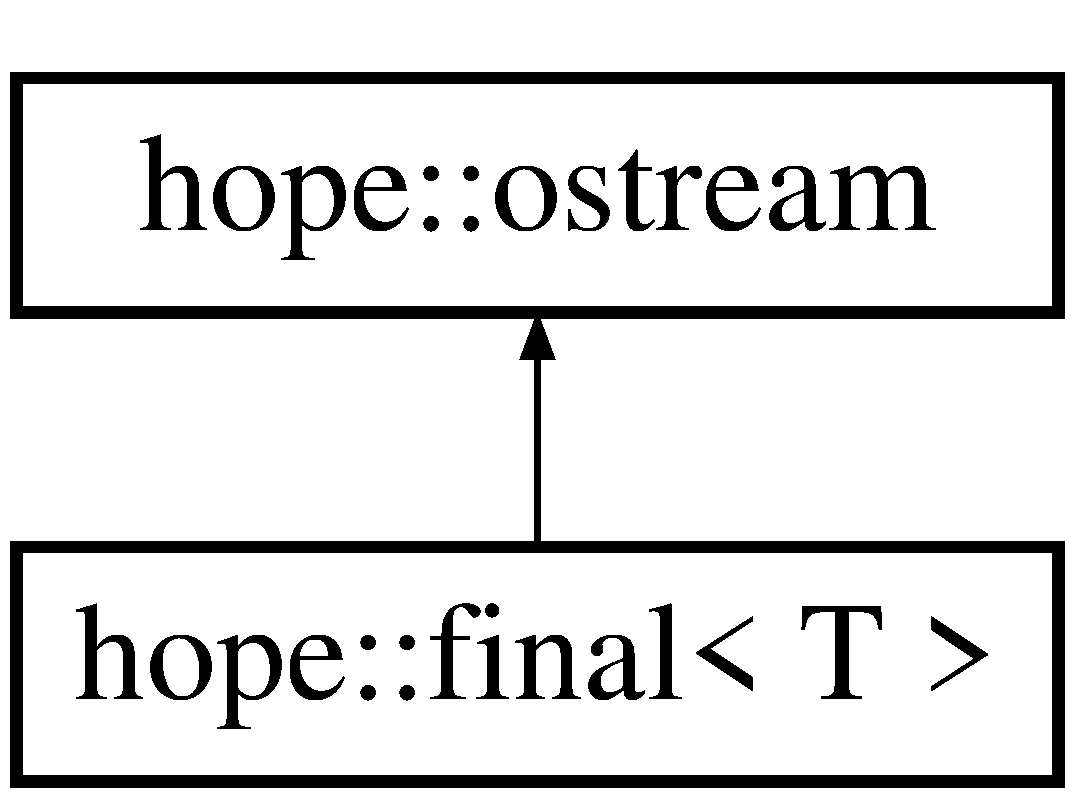
\includegraphics[height=2cm]{classhope_1_1final}
\end{center}
\end{figure}
\subsection*{Classes}
\begin{CompactItemize}
\item 
struct \textbf{final}
\begin{CompactList}\small\item\em Policy, used to specify how to convert struct to tuple. If instance of this structure is used, all the fields from an object will be copied to the tuple. \item\end{CompactList}\end{CompactItemize}
\subsection*{Public Member Functions}
\begin{CompactItemize}
\item 
\hypertarget{classhope_1_1final_0975f59458d62215cbaf0e69c4cc937c}{
{\footnotesize template$<$typename T $>$ }\\\textbf{fixed\_\-any} (T \&\&val)}
\label{classhope_1_1final_0975f59458d62215cbaf0e69c4cc937c}

\item 
\hypertarget{classhope_1_1final_e325e53d4738f0c8228b11c3dceb70e2}{
{\footnotesize template$<$typename T $>$ }\\const T \& \textbf{get} () const }
\label{classhope_1_1final_e325e53d4738f0c8228b11c3dceb70e2}

\item 
\hypertarget{classhope_1_1final_1c7929ca77ce3a3edc9c554fe9080463}{
{\footnotesize template$<$typename T $>$ }\\T \& \textbf{get} ()}
\label{classhope_1_1final_1c7929ca77ce3a3edc9c554fe9080463}

\item 
\hypertarget{classhope_1_1final_e61301b86f3346e0690e983cdbd595d5}{
\textbf{nonesuch} ()}
\label{classhope_1_1final_e61301b86f3346e0690e983cdbd595d5}

\item 
\hypertarget{classhope_1_1final_b05b8c165d7459649e2328b3f878bad2}{
\textbf{nonesuch} (nonesuch const \&)}
\label{classhope_1_1final_b05b8c165d7459649e2328b3f878bad2}

\item 
\hypertarget{classhope_1_1final_275c7f0352a663922e3c2b6a36e521cf}{
void \textbf{operator=} (nonesuch const \&)}
\label{classhope_1_1final_275c7f0352a663922e3c2b6a36e521cf}

\item 
\hypertarget{classhope_1_1final_45011c8067ecc50c4482d3bc98597b93}{
\textbf{factory} ()}
\label{classhope_1_1final_45011c8067ecc50c4482d3bc98597b93}

\item 
\hypertarget{classhope_1_1final_3095d86896dfed9f34941e0c84644b7f}{
\textbf{factory} (const factory \&)}
\label{classhope_1_1final_3095d86896dfed9f34941e0c84644b7f}

\item 
\hypertarget{classhope_1_1final_f33b5129efa38dd78067646df5f41acd}{
factory \& \textbf{operator=} (const factory \&)}
\label{classhope_1_1final_f33b5129efa38dd78067646df5f41acd}

\item 
\hypertarget{classhope_1_1final_f7035852a144dcc1bb3b5cf8cd52707b}{
{\footnotesize template$<$typename Type $>$ }\\bool \textbf{register\_\-object} (NameClass name)}
\label{classhope_1_1final_f7035852a144dcc1bb3b5cf8cd52707b}

\item 
\hypertarget{classhope_1_1final_032105ac5bedbf8b4b6cf2ba9d95966e}{
ReturnType $\ast$ \textbf{create} (const NameClass \&name) const }
\label{classhope_1_1final_032105ac5bedbf8b4b6cf2ba9d95966e}

\item 
\hypertarget{classhope_1_1final_56edd0c19d9298493ad5029abf87ba56}{
{\footnotesize template$<$typename... Ts$>$ }\\\textbf{fast\_\-pimpl} (Ts \&\&...args)}
\label{classhope_1_1final_56edd0c19d9298493ad5029abf87ba56}

\item 
\hypertarget{classhope_1_1final_cc44bc2eea7e247cf2d7bcb57f7649d7}{
T $\ast$ \textbf{operator $\rightarrow$ } () noexcept}
\label{classhope_1_1final_cc44bc2eea7e247cf2d7bcb57f7649d7}

\item 
\hypertarget{classhope_1_1final_71cd9a35eadcbae6440af54ae9213a34}{
const T $\ast$ \textbf{operator $\rightarrow$ } () const noexcept}
\label{classhope_1_1final_71cd9a35eadcbae6440af54ae9213a34}

\item 
\hypertarget{classhope_1_1final_b2f4e4e314182e3b906065cde61af2f5}{
T \& \textbf{operator=} (const T \&rhs) noexcept}
\label{classhope_1_1final_b2f4e4e314182e3b906065cde61af2f5}

\item 
\hypertarget{classhope_1_1final_e91c6193d80043db1a43bd9e98845873}{
T \& \textbf{operator$\ast$} () noexcept}
\label{classhope_1_1final_e91c6193d80043db1a43bd9e98845873}

\item 
\hypertarget{classhope_1_1final_69f5ec2a89be50ffb59b53484b098acd}{
const T \& \textbf{operator$\ast$} () const noexcept}
\label{classhope_1_1final_69f5ec2a89be50ffb59b53484b098acd}

\item 
\hypertarget{classhope_1_1final_bc99257f2062074fff841ff29afaaba0}{
\textbf{link\_\-holder\_\-array} ()}
\label{classhope_1_1final_bc99257f2062074fff841ff29afaaba0}

\item 
\hypertarget{classhope_1_1final_cc0466258e5dbbd500292d18124bed63}{
{\footnotesize template$<$typename T $>$ }\\constexpr T $\ast$ \textbf{get} () const noexcept}
\label{classhope_1_1final_cc0466258e5dbbd500292d18124bed63}

\item 
\hypertarget{classhope_1_1final_5f2f7125384b9e74fc35d40afc0f8d6b}{
bool \textbf{add} (BaseType $\ast$link) noexcept}
\label{classhope_1_1final_5f2f7125384b9e74fc35d40afc0f8d6b}

\item 
\hypertarget{classhope_1_1final_dce2583efb9eb6e93ecdccd2ada2e2de}{
bool \textbf{remove} (BaseType $\ast$link) noexcept}
\label{classhope_1_1final_dce2583efb9eb6e93ecdccd2ada2e2de}

\item 
\hypertarget{classhope_1_1final_8640643d923a3f7f3083a66c2b77a280}{
link\_\-list \& \textbf{get\_\-links} () noexcept}
\label{classhope_1_1final_8640643d923a3f7f3083a66c2b77a280}

\item 
\hypertarget{classhope_1_1final_7fd4e7675820ba8da52fdcf2ddf41492}{
const link\_\-list \& \textbf{get\_\-links} () const noexcept}
\label{classhope_1_1final_7fd4e7675820ba8da52fdcf2ddf41492}

\item 
\hypertarget{classhope_1_1final_303acd0d7275ea3eb7ea8b2e9d855bed}{
\textbf{link\_\-holder\_\-array} (const link\_\-holder\_\-array \&)}
\label{classhope_1_1final_303acd0d7275ea3eb7ea8b2e9d855bed}

\item 
\hypertarget{classhope_1_1final_106655976208aa4c9c84a7151d5ce815}{
\textbf{link\_\-holder\_\-array} (link\_\-holder\_\-array \&\&)}
\label{classhope_1_1final_106655976208aa4c9c84a7151d5ce815}

\item 
\hypertarget{classhope_1_1final_49c24958cc977efdd1cbe99ba25ff7e5}{
link\_\-holder\_\-array \& \textbf{operator=} (const link\_\-holder\_\-array \&)}
\label{classhope_1_1final_49c24958cc977efdd1cbe99ba25ff7e5}

\item 
\hypertarget{classhope_1_1final_007d11c443d70a175816889e952ab072}{
link\_\-holder\_\-array \& \textbf{operator=} (link\_\-holder\_\-array \&\&)}
\label{classhope_1_1final_007d11c443d70a175816889e952ab072}

\item 
\hypertarget{classhope_1_1final_d635a46d34aa5a332d98d55c55386930}{
\textbf{link\_\-holder\_\-tuple} ()}
\label{classhope_1_1final_d635a46d34aa5a332d98d55c55386930}

\item 
\hypertarget{classhope_1_1final_7a903b6f02dbcfa1059efe99faee0ab2}{
{\footnotesize template$<$typename T , typename NativeT  = std::decay\_\-t$<$T$>$$>$ }\\constexpr \textbf{decltype} (auto) get() const noexcept}
\label{classhope_1_1final_7a903b6f02dbcfa1059efe99faee0ab2}

\item 
\hypertarget{classhope_1_1final_6c07e673a719b0199b453793474e1541}{
{\footnotesize template$<$typename T $>$ }\\bool \textbf{add} (T $\ast$link) noexcept}
\label{classhope_1_1final_6c07e673a719b0199b453793474e1541}

\item 
\hypertarget{classhope_1_1final_cf1c04b8b370dc700f287be4d307ab2b}{
{\footnotesize template$<$typename T $>$ }\\bool \textbf{remove} (T $\ast$link) noexcept}
\label{classhope_1_1final_cf1c04b8b370dc700f287be4d307ab2b}

\item 
\hypertarget{classhope_1_1final_84ea3e2852e3692b63a95b78c197ab7f}{
\textbf{link\_\-holder\_\-tuple} (const link\_\-holder\_\-tuple \&)}
\label{classhope_1_1final_84ea3e2852e3692b63a95b78c197ab7f}

\item 
\hypertarget{classhope_1_1final_2c54b8c9263dee663cb0a51ea30cb4f3}{
\textbf{link\_\-holder\_\-tuple} (link\_\-holder\_\-tuple \&\&)}
\label{classhope_1_1final_2c54b8c9263dee663cb0a51ea30cb4f3}

\item 
\hypertarget{classhope_1_1final_c1176c101f3185f84a652638ab9c82b7}{
link\_\-holder\_\-tuple \& \textbf{operator=} (const link\_\-holder\_\-tuple \&)}
\label{classhope_1_1final_c1176c101f3185f84a652638ab9c82b7}

\item 
\hypertarget{classhope_1_1final_5229cb5247ce9273934f88136863683f}{
link\_\-holder\_\-tuple \& \textbf{operator=} (link\_\-holder\_\-tuple \&\&)}
\label{classhope_1_1final_5229cb5247ce9273934f88136863683f}

\item 
\hypertarget{classhope_1_1final_4e993ebfa25c6ab2bc6d5cb28f711512}{
\textbf{singleton\_\-holder} ()}
\label{classhope_1_1final_4e993ebfa25c6ab2bc6d5cb28f711512}

\item 
\hypertarget{classhope_1_1final_af516db9bbd8b80534adec0aa9bf8d65}{
\textbf{singleton\_\-holder} (singleton\_\-holder \&\&)}
\label{classhope_1_1final_af516db9bbd8b80534adec0aa9bf8d65}

\item 
\hypertarget{classhope_1_1final_3ad67d8e2a660cde191dda2952ace147}{
singleton\_\-holder \& \textbf{operator=} (singleton\_\-holder \&\&)}
\label{classhope_1_1final_3ad67d8e2a660cde191dda2952ace147}

\item 
\hypertarget{classhope_1_1final_245639ede2861e7b5b6c2805ba197613}{
constexpr \textbf{static\_\-string} (const char(\&str)\mbox{[}N\mbox{]})}
\label{classhope_1_1final_245639ede2861e7b5b6c2805ba197613}

\item 
\hypertarget{classhope_1_1final_b9c30670e6c38678195a944927d2002b}{
\textbf{switch\_\-expression} (const Key \&key)}
\label{classhope_1_1final_b9c30670e6c38678195a944927d2002b}

\item 
\hypertarget{classhope_1_1final_25122ddad9b9e375d02cc9df348d8c7f}{
key\_\-value\_\-pair \textbf{operator\mbox{[}$\,$\mbox{]}} (const Key \&key)}
\label{classhope_1_1final_25122ddad9b9e375d02cc9df348d8c7f}

\item 
\hypertarget{classhope_1_1final_de0143de1670994b815944b87ee610ce}{
{\footnotesize template$<$typename... Vs$>$ }\\constexpr \textbf{all} (Vs \&\&...args) noexcept}
\label{classhope_1_1final_de0143de1670994b815944b87ee610ce}

\item 
\hypertarget{classhope_1_1final_4ec0c84ee90b35265693bcfff1e3dd38}{
{\footnotesize template$<$typename T $>$ }\\constexpr bool \textbf{operator==} (const T \&rhs) const noexcept}
\label{classhope_1_1final_4ec0c84ee90b35265693bcfff1e3dd38}

\item 
\hypertarget{classhope_1_1final_4b5cc4ae2e43b62d9158d81c4f006f04}{
{\footnotesize template$<$typename T $>$ }\\constexpr bool \textbf{operator!=} (const T \&rhs) const noexcept}
\label{classhope_1_1final_4b5cc4ae2e43b62d9158d81c4f006f04}

\item 
\hypertarget{classhope_1_1final_b0bf99768bae97bd34580689228a494a}{
{\footnotesize template$<$typename... Vs$>$ }\\constexpr \textbf{any} (Vs \&\&...args) noexcept}
\label{classhope_1_1final_b0bf99768bae97bd34580689228a494a}

\item 
\hypertarget{classhope_1_1final_4ec0c84ee90b35265693bcfff1e3dd38}{
{\footnotesize template$<$typename T $>$ }\\constexpr bool \textbf{operator==} (const T \&rhs) const noexcept}
\label{classhope_1_1final_4ec0c84ee90b35265693bcfff1e3dd38}

\item 
\hypertarget{classhope_1_1final_4b5cc4ae2e43b62d9158d81c4f006f04}{
{\footnotesize template$<$typename T $>$ }\\constexpr bool \textbf{operator!=} (const T \&rhs) const noexcept}
\label{classhope_1_1final_4b5cc4ae2e43b62d9158d81c4f006f04}

\item 
\hypertarget{classhope_1_1final_aa957103cc4e6eb1d1587f4661b156e3}{
\textbf{log\_\-helper} (logger \&logger\_\-instance, log\_\-priority priority)}
\label{classhope_1_1final_aa957103cc4e6eb1d1587f4661b156e3}

\item 
\hypertarget{classhope_1_1final_43d3abf0a86be5751c9bcb5f121a43d8}{
\textbf{DECLARE\_\-NON\_\-MOVABLE} (logger)}
\label{classhope_1_1final_43d3abf0a86be5751c9bcb5f121a43d8}

\item 
\hypertarget{classhope_1_1final_7f42494e735fa3d7bfb969e945523987}{
\textbf{DECLARE\_\-NON\_\-COPYABLE} (logger)}
\label{classhope_1_1final_7f42494e735fa3d7bfb969e945523987}

\item 
\hypertarget{classhope_1_1final_76c2c3b7f0d8a66c818712b363c4e0d7}{
\textbf{logger} ()}
\label{classhope_1_1final_76c2c3b7f0d8a66c818712b363c4e0d7}

\item 
\hypertarget{classhope_1_1final_47b1e969a1eaca3c57b6b64bd0ddedab}{
bool \textbf{should\_\-write} (log\_\-priority priority) const noexcept}
\label{classhope_1_1final_47b1e969a1eaca3c57b6b64bd0ddedab}

\item 
\hypertarget{classhope_1_1final_49380a5aeb332d35a7bad7c86eec1ec2}{
void \textbf{enable} (ostream \&stream, log\_\-level level) noexcept}
\label{classhope_1_1final_49380a5aeb332d35a7bad7c86eec1ec2}

\item 
\hypertarget{classhope_1_1final_d84e14f532b5943dc5330c604ea26e59}{
\textbf{ofstream} (std::string\_\-view file\_\-name)}
\label{classhope_1_1final_d84e14f532b5943dc5330c604ea26e59}

\item 
\hypertarget{classhope_1_1final_e7e5b0b60acb8d4b0eb14cf96f54d76b}{
\textbf{DECLARE\_\-EXPLICIT\_\-DEFAULT\_\-MOVABLE} (ofstream)}
\label{classhope_1_1final_e7e5b0b60acb8d4b0eb14cf96f54d76b}

\item 
\hypertarget{classhope_1_1final_326e577f49062cd597bbcc630d38cbaf}{
\textbf{DECLARE\_\-NON\_\-COPYABLE} (ofstream)}
\label{classhope_1_1final_326e577f49062cd597bbcc630d38cbaf}

\item 
\hypertarget{classhope_1_1final_353197e5aca45505be10a0d238a2450b}{
virtual bool \textbf{is\_\-open} () const noexcept override}
\label{classhope_1_1final_353197e5aca45505be10a0d238a2450b}

\item 
\hypertarget{classhope_1_1final_2807c24032cbd21e31befc6b57b0f323}{
virtual void \textbf{write} (const void $\ast$data, std::size\_\-t size) override}
\label{classhope_1_1final_2807c24032cbd21e31befc6b57b0f323}

\item 
\hypertarget{classhope_1_1final_497bcdd6f4bd42b42394a96fec40dba8}{
virtual void \textbf{flush} () override}
\label{classhope_1_1final_497bcdd6f4bd42b42394a96fec40dba8}

\item 
\hypertarget{classhope_1_1final_f2287f80ed00ea759d6b536f3833e1ac}{
\textbf{stack\_\-buffer} ()}
\label{classhope_1_1final_f2287f80ed00ea759d6b536f3833e1ac}

\item 
\hypertarget{classhope_1_1final_c796477284de807d7005387efb105ef0}{
\textbf{DECLARE\_\-NON\_\-MOVABLE} (stack\_\-buffer)}
\label{classhope_1_1final_c796477284de807d7005387efb105ef0}

\item 
\hypertarget{classhope_1_1final_09fdce3a73ab9d34e18ab28a3b5610d4}{
\textbf{DECLARE\_\-NON\_\-COPYABLE} (stack\_\-buffer)}
\label{classhope_1_1final_09fdce3a73ab9d34e18ab28a3b5610d4}

\item 
\hypertarget{classhope_1_1final_72637e3e00e19fbb398bfaf29b548463}{
void \textbf{put} (const void $\ast$data, std::size\_\-t size) noexcept}
\label{classhope_1_1final_72637e3e00e19fbb398bfaf29b548463}

\item 
\hypertarget{classhope_1_1final_3c9415ea9f20efe10be3464183e51592}{
{\footnotesize template$<$typename... VTs, typename  = std::enable\_\-if\_\-t$<$std::is\_\-same\_\-v$<$type\_\-list$<$std::decay\_\-t$<$VTs$>$...$>$, type\_\-list$<$std::decay\_\-t$<$Ts$>$...$>$$>$$>$$>$ }\\constexpr \textbf{flat\_\-tuple} (VTs \&\&...elems) noexcept}
\label{classhope_1_1final_3c9415ea9f20efe10be3464183e51592}

\item 
\hypertarget{classhope_1_1final_e9774b7f26cb585b5ef83deb5a341b3c}{
constexpr \textbf{flat\_\-tuple} ()}
\label{classhope_1_1final_e9774b7f26cb585b5ef83deb5a341b3c}

\item 
\hypertarget{classhope_1_1final_2f01a7839847713939813c9f6d5ff315}{
constexpr std::size\_\-t \textbf{operator()} (const flat\_\-tuple$<$ Ts...$>$ \&tuple)}
\label{classhope_1_1final_2f01a7839847713939813c9f6d5ff315}

\item 
\hypertarget{classhope_1_1final_6634fff470139a5e8afde02afa1bd9ef}{
\textbf{variant} ()}
\label{classhope_1_1final_6634fff470139a5e8afde02afa1bd9ef}

\item 
\hypertarget{classhope_1_1final_3aac7a012a2890ce74ff8bcfdda253fb}{
{\footnotesize template$<$typename T $>$ }\\\textbf{variant} (T \&\&type)}
\label{classhope_1_1final_3aac7a012a2890ce74ff8bcfdda253fb}

\item 
\hypertarget{classhope_1_1final_97372acb21ea0b5e13f92266a6a02e2c}{
{\footnotesize template$<$typename T $>$ }\\variant \& \textbf{operator=} (T \&\&value)}
\label{classhope_1_1final_97372acb21ea0b5e13f92266a6a02e2c}

\item 
\hypertarget{classhope_1_1final_1c7929ca77ce3a3edc9c554fe9080463}{
{\footnotesize template$<$typename T $>$ }\\T \& \textbf{get} ()}
\label{classhope_1_1final_1c7929ca77ce3a3edc9c554fe9080463}

\end{CompactItemize}
\subsection*{Static Public Member Functions}
\begin{CompactItemize}
\item 
\hypertarget{classhope_1_1final_13b450c504d01d7bfc33fc4692d0fa80}{
static SingletonImpl $\ast$ \textbf{create} ()}
\label{classhope_1_1final_13b450c504d01d7bfc33fc4692d0fa80}

\item 
\hypertarget{classhope_1_1final_5b08245700881f722aee4811b62e6aec}{
static void \textbf{destroy} (SingletonImpl $\ast$instance)}
\label{classhope_1_1final_5b08245700881f722aee4811b62e6aec}

\item 
\hypertarget{classhope_1_1final_13b450c504d01d7bfc33fc4692d0fa80}{
static SingletonImpl $\ast$ \textbf{create} ()}
\label{classhope_1_1final_13b450c504d01d7bfc33fc4692d0fa80}

\item 
\hypertarget{classhope_1_1final_5b08245700881f722aee4811b62e6aec}{
static void \textbf{destroy} (SingletonImpl $\ast$instance)}
\label{classhope_1_1final_5b08245700881f722aee4811b62e6aec}

\item 
\hypertarget{classhope_1_1final_268efe68664b71ead7fb1bcf838bb51f}{
static void \textbf{on\_\-dead\_\-reference} ()}
\label{classhope_1_1final_268efe68664b71ead7fb1bcf838bb51f}

\item 
\hypertarget{classhope_1_1final_00be6ae22eb41e3315e169c26a19e5cf}{
static void \textbf{register\_\-deleter} (detail::Deleter deleter)}
\label{classhope_1_1final_00be6ae22eb41e3315e169c26a19e5cf}

\item 
\hypertarget{classhope_1_1final_268efe68664b71ead7fb1bcf838bb51f}{
static void \textbf{on\_\-dead\_\-reference} ()}
\label{classhope_1_1final_268efe68664b71ead7fb1bcf838bb51f}

\item 
\hypertarget{classhope_1_1final_00be6ae22eb41e3315e169c26a19e5cf}{
static void \textbf{register\_\-deleter} (detail::Deleter deleter)}
\label{classhope_1_1final_00be6ae22eb41e3315e169c26a19e5cf}

\item 
\hypertarget{classhope_1_1final_268efe68664b71ead7fb1bcf838bb51f}{
static void \textbf{on\_\-dead\_\-reference} ()}
\label{classhope_1_1final_268efe68664b71ead7fb1bcf838bb51f}

\item 
\hypertarget{classhope_1_1final_00be6ae22eb41e3315e169c26a19e5cf}{
static void \textbf{register\_\-deleter} (detail::Deleter deleter)}
\label{classhope_1_1final_00be6ae22eb41e3315e169c26a19e5cf}

\item 
\hypertarget{classhope_1_1final_268efe68664b71ead7fb1bcf838bb51f}{
static void \textbf{on\_\-dead\_\-reference} ()}
\label{classhope_1_1final_268efe68664b71ead7fb1bcf838bb51f}

\item 
\hypertarget{classhope_1_1final_00be6ae22eb41e3315e169c26a19e5cf}{
static void \textbf{register\_\-deleter} (detail::Deleter deleter)}
\label{classhope_1_1final_00be6ae22eb41e3315e169c26a19e5cf}

\item 
\hypertarget{classhope_1_1final_715040978b295bca11bd5f396377b138}{
static SingletonImpl \& \textbf{instance} ()}
\label{classhope_1_1final_715040978b295bca11bd5f396377b138}

\item 
\hypertarget{classhope_1_1final_8a5bdf6cd1e21c29f1e3cd9b41fa8d9b}{
{\footnotesize template$<$typename Key $>$ }\\static constexpr auto \textbf{get} () noexcept}
\label{classhope_1_1final_8a5bdf6cd1e21c29f1e3cd9b41fa8d9b}

\item 
{\footnotesize template$<$typename T $>$ }\\static value\_\-wrapper$<$ T $>$ \hyperlink{classhope_1_1final_3c394b218c24c4d9795f84c1d1f0bf2d}{build\_\-value} (const T \&value)
\end{CompactItemize}
\subsection*{Public Attributes}
\begin{CompactItemize}
\item 
\hypertarget{classhope_1_1final_4b912feec93db9aaa7802f82e293d3ae}{
char \textbf{value} \mbox{[}N\mbox{]}}
\label{classhope_1_1final_4b912feec93db9aaa7802f82e293d3ae}

\item 
\hypertarget{classhope_1_1final_c3a87c4cd07b4996bad0ebb85181411b}{
std::size\_\-t \textbf{bytes\_\-written} = 0}
\label{classhope_1_1final_c3a87c4cd07b4996bad0ebb85181411b}

\item 
\hypertarget{classhope_1_1final_43ea140ced19b04247964ae77c219b03}{
buffer\_\-t \textbf{buffer}}
\label{classhope_1_1final_43ea140ced19b04247964ae77c219b03}

\item 
\hypertarget{classhope_1_1final_2d91342662d625ab9acac0ba32f8aaa5}{
std::vector$<$ char $>$ \textbf{additional\_\-buffer}}
\label{classhope_1_1final_2d91342662d625ab9acac0ba32f8aaa5}

\end{CompactItemize}
\subsection*{Static Public Attributes}
\begin{CompactItemize}
\item 
\hypertarget{classhope_1_1final_956a53f1be43cefc4ec367bb59d93741}{
static constexpr std::size\_\-t \textbf{BufferSize} = 1023}
\label{classhope_1_1final_956a53f1be43cefc4ec367bb59d93741}

\end{CompactItemize}
\subsection*{Friends}
\begin{CompactItemize}
\item 
\hypertarget{classhope_1_1final_d8937554df8f60f7d5a139a6e1cdf30c}{
class \textbf{LifetimeModel$<$ SingletonImpl $>$}}
\label{classhope_1_1final_d8937554df8f60f7d5a139a6e1cdf30c}

\item 
\hypertarget{classhope_1_1final_d4eb20df876e902e975bf963da1ccf3e}{
class \textbf{key\_\-value\_\-pair}}
\label{classhope_1_1final_d4eb20df876e902e975bf963da1ccf3e}

\item 
\hypertarget{classhope_1_1final_062105058b490688776712c2f521b652}{
struct \textbf{log\_\-helper}}
\label{classhope_1_1final_062105058b490688776712c2f521b652}

\item 
\hypertarget{classhope_1_1final_da168e37d00bf11194fa7af409a23e2f}{
{\footnotesize template$<$typename T $>$ }\\constexpr bool \textbf{operator==} (const T \&lhs, const all \&rhs) noexcept}
\label{classhope_1_1final_da168e37d00bf11194fa7af409a23e2f}

\item 
\hypertarget{classhope_1_1final_4c9701d52b4c887172d578270d0ef889}{
{\footnotesize template$<$typename T $>$ }\\constexpr bool \textbf{operator!=} (const T \&lhs, const all \&rhs) noexcept}
\label{classhope_1_1final_4c9701d52b4c887172d578270d0ef889}

\item 
\hypertarget{classhope_1_1final_352e0f1c775282fed9323e1606d74f15}{
{\footnotesize template$<$typename T $>$ }\\constexpr bool \textbf{operator==} (const T \&lhs, const any \&rhs) noexcept}
\label{classhope_1_1final_352e0f1c775282fed9323e1606d74f15}

\item 
\hypertarget{classhope_1_1final_2c688c778ddbcaf0f12f719776c42ebf}{
{\footnotesize template$<$typename T $>$ }\\constexpr bool \textbf{operator!=} (const T \&lhs, const any \&rhs) noexcept}
\label{classhope_1_1final_2c688c778ddbcaf0f12f719776c42ebf}

\item 
{\footnotesize template$<$typename T $>$ }\\log\_\-helper \& \hyperlink{classhope_1_1final_4b8322ee0fd5ae2a2a0a9052876e6f8d}{operator$<$$<$} (log\_\-helper \&helper, const T \&value)
\item 
{\footnotesize template$<$typename T $>$ }\\log\_\-helper \& \hyperlink{classhope_1_1final_e477d848d5b78d071e802988f5d72584}{operator$<$$<$} (log\_\-helper \&\&helper, const T \&value)
\end{CompactItemize}


\subsection{Detailed Description}
\subsubsection*{template$<$typename T$>$ class hope::final$<$ T $>$}

Implementation of the struct like non recursive tuple which might be used to directly cast to struct with same fields because alignment of the structs's fields and tuple's fields are match. 

struct used as namespace to policies which is used for tuple creation functions

Helper class for log writing, provide dispatch of the writing value according their type

\begin{Desc}
\item[Template Parameters:]
\begin{description}
\item[{\em Ts}]types which might be stored in the tuple \end{description}
\end{Desc}


\subsection{Member Function Documentation}
\hypertarget{classhope_1_1final_3c394b218c24c4d9795f84c1d1f0bf2d}{
\index{hope::final@{hope::final}!build\_\-value@{build\_\-value}}
\index{build\_\-value@{build\_\-value}!hope::final@{hope::final}}
\subsubsection[{build\_\-value}]{\setlength{\rightskip}{0pt plus 5cm}template$<$typename T $>$ template$<$typename T $>$ static value\_\-wrapper$<$T$>$ {\bf hope::final}$<$ T $>$::build\_\-value (const T \& {\em value})\hspace{0.3cm}{\tt  \mbox{[}inline, static\mbox{]}}}}
\label{classhope_1_1final_3c394b218c24c4d9795f84c1d1f0bf2d}


Wrap value to store it with pretty form: \mbox{[}VALUE\mbox{]} 

\subsection{Friends And Related Function Documentation}
\hypertarget{classhope_1_1final_e477d848d5b78d071e802988f5d72584}{
\index{hope::final@{hope::final}!operator$<$$<$@{operator$<$$<$}}
\index{operator$<$$<$@{operator$<$$<$}!hope::final@{hope::final}}
\subsubsection[{operator$<$$<$}]{\setlength{\rightskip}{0pt plus 5cm}template$<$typename T $>$ template$<$typename T $>$ log\_\-helper\& operator$<$$<$ (log\_\-helper \&\& {\em helper}, \/  const T \& {\em value})\hspace{0.3cm}{\tt  \mbox{[}friend\mbox{]}}}}
\label{classhope_1_1final_e477d848d5b78d071e802988f5d72584}


Function needed to delegate call to the same operator$<$$<$, but with a little different semantic On MSVC it does not need, but another compilers can not call function with non const reference parameter with rvalue \hypertarget{classhope_1_1final_4b8322ee0fd5ae2a2a0a9052876e6f8d}{
\index{hope::final@{hope::final}!operator$<$$<$@{operator$<$$<$}}
\index{operator$<$$<$@{operator$<$$<$}!hope::final@{hope::final}}
\subsubsection[{operator$<$$<$}]{\setlength{\rightskip}{0pt plus 5cm}template$<$typename T $>$ template$<$typename T $>$ log\_\-helper\& operator$<$$<$ (log\_\-helper \& {\em helper}, \/  const T \& {\em value})\hspace{0.3cm}{\tt  \mbox{[}friend\mbox{]}}}}
\label{classhope_1_1final_4b8322ee0fd5ae2a2a0a9052876e6f8d}


Central point of writing operation, provide type dispatch and call desired write method. If the type is enum and write\_\-enum had been detected, thus it will be called If member function with signature void write(log\_\-helper\&) detected, it will be called If global function with signature void write(log\_\-helper, const T\&) detected, it will be called \begin{Desc}
\item[Template Parameters:]
\begin{description}
\item[{\em T}]Type of th eobject to be written \end{description}
\end{Desc}
\begin{Desc}
\item[Parameters:]
\begin{description}
\item[{\em helper}]Self \item[{\em value}]Instance of the object to be written \end{description}
\end{Desc}
\begin{Desc}
\item[Returns:]Self \end{Desc}


The documentation for this class was generated from the following files:\begin{CompactItemize}
\item 
lib/hope/any/fixed\_\-any.h\item 
lib/hope/components/factory.h\item 
lib/hope/components/singleton\_\-holder/singleton\_\-holder.h\item 
lib/hope/components/static\_\-string.h\item 
lib/hope/components/switch\_\-expression/switch\_\-expression.h\item 
lib/hope/components/utility.h\item 
lib/hope/logger/log\_\-helper.h\item 
lib/hope/logger/logger.h\item 
lib/hope/logger/ofstream.h\item 
lib/hope/logger/stack\_\-buffer.h\item 
lib/hope/variant/variant.hpp\item 
lib/hope/components/detector.h\item 
lib/hope/components/fast\_\-pimpl.h\item 
lib/hope/components/link\_\-holder/link\_\-holder\_\-array.h\item 
lib/hope/components/link\_\-holder/link\_\-holder\_\-tuple.h\item 
lib/hope/components/singleton\_\-holder/creation\_\-model.h\item 
lib/hope/components/singleton\_\-holder/lifetime\_\-model.h\item 
lib/hope/components/typemap.h\item 
lib/hope/tuple/\hyperlink{flat__tuple_8h}{flat\_\-tuple.h}\item 
lib/hope/tuple/tuple\_\-utils.h\end{CompactItemize}

\hypertarget{structhope_1_1memory_1_1final}{
\section{hope::memory::final Class Reference}
\label{structhope_1_1memory_1_1final}\index{hope::memory::final@{hope::memory::final}}
}
Low level chunk allocator, is made such as tricky linked list first byte of the chunks block stores position of the next available element, thus we try to avoid extra memory utilization, also chunk knows nothing about it's block size, therefore alloc and dealloc methods looks so strange (their signature contain related params...) but it is worth remembering that chunk can't allocate blocks with different sizes.  


{\tt \#include $<$chunk.h$>$}

\subsection*{Public Member Functions}
\begin{CompactItemize}
\item 
void \hyperlink{structhope_1_1memory_1_1final_4ceb422bbc652ee386c8458abc959425}{init} (std::size\_\-t block\_\-size, uint8\_\-t blocks\_\-count) noexcept
\begin{CompactList}\small\item\em I decide to do not use RAII principle, to avoid any explicit constructors chunk should be as simple struct as possible, btw it is lowest level in allocation hierarchy. \item\end{CompactList}\item 
void $\ast$ \hyperlink{structhope_1_1memory_1_1final_6b0b52dcc62d04aa1a8c3bb6168a7ce4}{allocate} (std::size\_\-t block\_\-size) noexcept
\begin{CompactList}\small\item\em Allocation of chunks block, block\_\-size is passed throw methods parameter, because it is too expensive to store this value at the chunk struct (due to the allocators hierarchy, see \hyperlink{fixed__allocator_8h-source}{fixed\_\-allocator.h} for more details) this method extract first available block from linked list, and do other related work, it is easy to understand. \item\end{CompactList}\item 
void \hyperlink{structhope_1_1memory_1_1final_9c7e918080a8c1429ec8d241e7dfe0cf}{deallocate} (void $\ast$ptr, std::size\_\-t block\_\-size) noexcept
\begin{CompactList}\small\item\em freed passed memory witch is related by the passed pointer \item\end{CompactList}\item 
bool \hyperlink{structhope_1_1memory_1_1final_180904dab84e90547c6664815c449416}{is\_\-deallocation\_\-valid} (void $\ast$ptr, std::size\_\-t block\_\-size) const noexcept
\begin{CompactList}\small\item\em checks if deallocation of passed ptr with passed value is available, otherwise we just cough memory corruption ot other invalid activity \item\end{CompactList}\item 
bool \hyperlink{structhope_1_1memory_1_1final_44c5aa574f7dea1a3689fdb6e1215bf1}{is\_\-allocation\_\-valid} (std::size\_\-t block\_\-size) const noexcept
\begin{CompactList}\small\item\em check if allocation of block currently available \item\end{CompactList}\item 
\hypertarget{structhope_1_1memory_1_1final_ca1fedc5f4cb9a16cd668f09cf0c5233}{
\textbf{fixed\_\-allocator} (uint8\_\-t max\_\-blocks\_\-count, std::size\_\-t block\_\-size) noexcept}
\label{structhope_1_1memory_1_1final_ca1fedc5f4cb9a16cd668f09cf0c5233}

\item 
\hypertarget{structhope_1_1memory_1_1final_bc3b393955cb128645dddaaa2e3a7cce}{
\textbf{fixed\_\-allocator} (fixed\_\-allocator \&\&rhs) noexcept}
\label{structhope_1_1memory_1_1final_bc3b393955cb128645dddaaa2e3a7cce}

\item 
\hypertarget{structhope_1_1memory_1_1final_b36950f24b55764a6a628803d53163c3}{
fixed\_\-allocator \& \textbf{operator=} (fixed\_\-allocator \&\&rhs) noexcept}
\label{structhope_1_1memory_1_1final_b36950f24b55764a6a628803d53163c3}

\item 
\hyperlink{structhope_1_1memory_1_1final_3e02f1cf966f5447a579d51afa98330c}{fixed\_\-allocator} (const fixed\_\-allocator \&rhs)
\begin{CompactList}\small\item\em to avoid extra or unsafe copying we have to explicitly delete copy constructor and copy assign operator also, we should create explicit noexcept move constructor and copy assign operator \item\end{CompactList}\item 
\hypertarget{structhope_1_1memory_1_1final_ce713dd85f29313a87f24eae31a5a809}{
fixed\_\-allocator \& \textbf{operator=} (const fixed\_\-allocator \&rhs)}
\label{structhope_1_1memory_1_1final_ce713dd85f29313a87f24eae31a5a809}

\item 
\hypertarget{structhope_1_1memory_1_1final_517c29298f9b737bce38f335df100461}{
void $\ast$ \hyperlink{structhope_1_1memory_1_1final_517c29298f9b737bce38f335df100461}{allocate} () noexcept}
\label{structhope_1_1memory_1_1final_517c29298f9b737bce38f335df100461}

\begin{CompactList}\small\item\em allocate block with m\_\-block\_\-size size \item\end{CompactList}\item 
\hypertarget{structhope_1_1memory_1_1final_da58e8008844f554080b7ebd9513035d}{
void \hyperlink{structhope_1_1memory_1_1final_da58e8008844f554080b7ebd9513035d}{deallocate} (void $\ast$ptr) noexcept}
\label{structhope_1_1memory_1_1final_da58e8008844f554080b7ebd9513035d}

\begin{CompactList}\small\item\em try to deallocate passed pointer, if it were allocated by another memory pool in debug this caused assert failure in realize mode this causes undefined behavior \item\end{CompactList}\item 
\hypertarget{structhope_1_1memory_1_1final_f6bf303e9162923afc80ef1b3081a1fa}{
std::size\_\-t \hyperlink{structhope_1_1memory_1_1final_f6bf303e9162923afc80ef1b3081a1fa}{block\_\-size} () const noexcept}
\label{structhope_1_1memory_1_1final_f6bf303e9162923afc80ef1b3081a1fa}

\begin{CompactList}\small\item\em returns size of block, witch may be allocated \item\end{CompactList}\item 
\hypertarget{structhope_1_1memory_1_1final_574fe43c8a88fab43e213dd568f1db78}{
\textbf{small\_\-object\_\-allocator} (const small\_\-object\_\-allocator \&)}
\label{structhope_1_1memory_1_1final_574fe43c8a88fab43e213dd568f1db78}

\item 
\hypertarget{structhope_1_1memory_1_1final_4e4c83e609c448a110754eb8b68c3096}{
\textbf{small\_\-object\_\-allocator} (small\_\-object\_\-allocator \&\&)}
\label{structhope_1_1memory_1_1final_4e4c83e609c448a110754eb8b68c3096}

\item 
\hypertarget{structhope_1_1memory_1_1final_6c1420340012d0490acff1905652b81c}{
small\_\-object\_\-allocator \& \textbf{operator=} (const small\_\-object\_\-allocator \&)}
\label{structhope_1_1memory_1_1final_6c1420340012d0490acff1905652b81c}

\item 
\hypertarget{structhope_1_1memory_1_1final_bfd98ecd6fb623123d8bf2870e696953}{
small\_\-object\_\-allocator \& \textbf{operator=} (small\_\-object\_\-allocator \&\&)}
\label{structhope_1_1memory_1_1final_bfd98ecd6fb623123d8bf2870e696953}

\item 
\hypertarget{structhope_1_1memory_1_1final_c4a6466c5b4eca5c9251eb4406540cb6}{
void \hyperlink{structhope_1_1memory_1_1final_c4a6466c5b4eca5c9251eb4406540cb6}{deallocate} (void $\ast$ptr, std::size\_\-t size) noexcept}
\label{structhope_1_1memory_1_1final_c4a6466c5b4eca5c9251eb4406540cb6}

\begin{CompactList}\small\item\em try to deallocate passed pointer to object since allocator is stateful, you cannot deallocate objects, which were allocated by this class params meaning are trivial \item\end{CompactList}\item 
\hypertarget{structhope_1_1memory_1_1final_ddd2a53238c4a13ac22734a0ff70e594}{
void $\ast$ \hyperlink{structhope_1_1memory_1_1final_ddd2a53238c4a13ac22734a0ff70e594}{allocate} (std::size\_\-t size) noexcept}
\label{structhope_1_1memory_1_1final_ddd2a53238c4a13ac22734a0ff70e594}

\begin{CompactList}\small\item\em try to allocate object, if passed size greater than m\_\-max\_\-object\_\-size, operator new will be called params meaning are trivial \item\end{CompactList}\end{CompactItemize}
\subsection*{Static Public Member Functions}
\begin{CompactItemize}
\item 
\hypertarget{structhope_1_1memory_1_1final_60ac0028ba156818940a7c7da2ba12e1}{
static small\_\-object\_\-allocator \& \hyperlink{structhope_1_1memory_1_1final_60ac0028ba156818940a7c7da2ba12e1}{instance} ()}
\label{structhope_1_1memory_1_1final_60ac0028ba156818940a7c7da2ba12e1}

\begin{CompactList}\small\item\em just return instance of singleton NOTE: before use this class, u have to initialize its instance, see small\_\-object\_\-allocator::initialize \item\end{CompactList}\end{CompactItemize}
\subsection*{Friends}
\begin{CompactItemize}
\item 
\hypertarget{structhope_1_1memory_1_1final_430993a05a9a34af3e25581753c4d24a}{
class \textbf{sm\_\-allocator\_\-reset}}
\label{structhope_1_1memory_1_1final_430993a05a9a34af3e25581753c4d24a}

\end{CompactItemize}


\subsection{Detailed Description}
Low level chunk allocator, is made such as tricky linked list first byte of the chunks block stores position of the next available element, thus we try to avoid extra memory utilization, also chunk knows nothing about it's block size, therefore alloc and dealloc methods looks so strange (their signature contain related params...) but it is worth remembering that chunk can't allocate blocks with different sizes. 

singleton, is used to hold list with fixed allocators of proper sizes 

\subsection{Member Function Documentation}
\hypertarget{structhope_1_1memory_1_1final_6b0b52dcc62d04aa1a8c3bb6168a7ce4}{
\index{hope::memory::final@{hope::memory::final}!allocate@{allocate}}
\index{allocate@{allocate}!hope::memory::final@{hope::memory::final}}
\subsubsection[{allocate}]{\setlength{\rightskip}{0pt plus 5cm}void$\ast$ hope::memory::final::allocate (std::size\_\-t {\em block\_\-size})}}
\label{structhope_1_1memory_1_1final_6b0b52dcc62d04aa1a8c3bb6168a7ce4}


Allocation of chunks block, block\_\-size is passed throw methods parameter, because it is too expensive to store this value at the chunk struct (due to the allocators hierarchy, see \hyperlink{fixed__allocator_8h-source}{fixed\_\-allocator.h} for more details) this method extract first available block from linked list, and do other related work, it is easy to understand. 

\begin{Desc}
\item[Parameters:]
\begin{description}
\item[{\em block\_\-size}]- size of block to be allocated \end{description}
\end{Desc}
\begin{Desc}
\item[Returns:]pointer to the desired memory segment \end{Desc}
\hypertarget{structhope_1_1memory_1_1final_9c7e918080a8c1429ec8d241e7dfe0cf}{
\index{hope::memory::final@{hope::memory::final}!deallocate@{deallocate}}
\index{deallocate@{deallocate}!hope::memory::final@{hope::memory::final}}
\subsubsection[{deallocate}]{\setlength{\rightskip}{0pt plus 5cm}void hope::memory::final::deallocate (void $\ast$ {\em ptr}, \/  std::size\_\-t {\em block\_\-size})}}
\label{structhope_1_1memory_1_1final_9c7e918080a8c1429ec8d241e7dfe0cf}


freed passed memory witch is related by the passed pointer 

\begin{Desc}
\item[Parameters:]
\begin{description}
\item[{\em ptr}]pointer to the memory block to be allocated, value should be in range of \mbox{[}data, data + block\_\-size $\ast$ blocks\_\-count\mbox{]} in other words this memory should be recently allocated from this chunk \item[{\em block\_\-size}]size of block to be freed \end{description}
\end{Desc}
\hypertarget{structhope_1_1memory_1_1final_3e02f1cf966f5447a579d51afa98330c}{
\index{hope::memory::final@{hope::memory::final}!fixed\_\-allocator@{fixed\_\-allocator}}
\index{fixed\_\-allocator@{fixed\_\-allocator}!hope::memory::final@{hope::memory::final}}
\subsubsection[{fixed\_\-allocator}]{\setlength{\rightskip}{0pt plus 5cm}hope::memory::final::fixed\_\-allocator (const fixed\_\-allocator \& {\em rhs})}}
\label{structhope_1_1memory_1_1final_3e02f1cf966f5447a579d51afa98330c}


to avoid extra or unsafe copying we have to explicitly delete copy constructor and copy assign operator also, we should create explicit noexcept move constructor and copy assign operator 

\begin{Desc}
\item[Parameters:]
\begin{description}
\item[{\em rhs}]\end{description}
\end{Desc}
\hypertarget{structhope_1_1memory_1_1final_4ceb422bbc652ee386c8458abc959425}{
\index{hope::memory::final@{hope::memory::final}!init@{init}}
\index{init@{init}!hope::memory::final@{hope::memory::final}}
\subsubsection[{init}]{\setlength{\rightskip}{0pt plus 5cm}void hope::memory::final::init (std::size\_\-t {\em block\_\-size}, \/  uint8\_\-t {\em blocks\_\-count})}}
\label{structhope_1_1memory_1_1final_4ceb422bbc652ee386c8458abc959425}


I decide to do not use RAII principle, to avoid any explicit constructors chunk should be as simple struct as possible, btw it is lowest level in allocation hierarchy. 

\begin{Desc}
\item[Parameters:]
\begin{description}
\item[{\em block\_\-size}]size of single block to be stored at the chunk; this is only one lock size which is available for allocation \item[{\em blocks\_\-count}]count of chunk's blocks to be allocated, value in range of \mbox{[}0, 255\mbox{]} this is most appropriate interval to avoid memory alignment falls (maximum available index of chunk block is 255 due to byte size) \end{description}
\end{Desc}
\hypertarget{structhope_1_1memory_1_1final_44c5aa574f7dea1a3689fdb6e1215bf1}{
\index{hope::memory::final@{hope::memory::final}!is\_\-allocation\_\-valid@{is\_\-allocation\_\-valid}}
\index{is\_\-allocation\_\-valid@{is\_\-allocation\_\-valid}!hope::memory::final@{hope::memory::final}}
\subsubsection[{is\_\-allocation\_\-valid}]{\setlength{\rightskip}{0pt plus 5cm}bool hope::memory::final::is\_\-allocation\_\-valid (std::size\_\-t {\em block\_\-size}) const}}
\label{structhope_1_1memory_1_1final_44c5aa574f7dea1a3689fdb6e1215bf1}


check if allocation of block currently available 

\begin{Desc}
\item[Parameters:]
\begin{description}
\item[{\em block\_\-size}]size of block to be allocated \end{description}
\end{Desc}
\begin{Desc}
\item[Returns:]true if allocation is possible \end{Desc}
\hypertarget{structhope_1_1memory_1_1final_180904dab84e90547c6664815c449416}{
\index{hope::memory::final@{hope::memory::final}!is\_\-deallocation\_\-valid@{is\_\-deallocation\_\-valid}}
\index{is\_\-deallocation\_\-valid@{is\_\-deallocation\_\-valid}!hope::memory::final@{hope::memory::final}}
\subsubsection[{is\_\-deallocation\_\-valid}]{\setlength{\rightskip}{0pt plus 5cm}bool hope::memory::final::is\_\-deallocation\_\-valid (void $\ast$ {\em ptr}, \/  std::size\_\-t {\em block\_\-size}) const}}
\label{structhope_1_1memory_1_1final_180904dab84e90547c6664815c449416}


checks if deallocation of passed ptr with passed value is available, otherwise we just cough memory corruption ot other invalid activity 

\begin{Desc}
\item[Parameters:]
\begin{description}
\item[{\em ptr}]pointer to the block to be deallocated \item[{\em block\_\-size}]size of deallocating block \end{description}
\end{Desc}
\begin{Desc}
\item[Returns:]true id deallocation may be successful, otherwise false \end{Desc}


The documentation for this class was generated from the following files:\begin{CompactItemize}
\item 
lib/hope/memory/small\_\-object/chunk.h\item 
lib/hope/memory/small\_\-object/fixed\_\-allocator.h\item 
lib/hope/memory/small\_\-object/small\_\-object\_\-allocator.h\end{CompactItemize}

\hypertarget{classhope_1_1detail_1_1flat__tuple__impl_3_01std_1_1index__sequence_3_01_is_8_8_8_4_00_01_ts_8_8_8_4}{
\section{hope::detail::flat\_\-tuple\_\-impl$<$ std::index\_\-sequence$<$ Is...$>$, Ts...$>$ Class Template Reference}
\label{classhope_1_1detail_1_1flat__tuple__impl_3_01std_1_1index__sequence_3_01_is_8_8_8_4_00_01_ts_8_8_8_4}\index{hope::detail::flat\_\-tuple\_\-impl$<$ std::index\_\-sequence$<$ Is...$>$, Ts...$>$@{hope::detail::flat\_\-tuple\_\-impl$<$ std::index\_\-sequence$<$ Is...$>$, Ts...$>$}}
}
{\tt \#include $<$flat\_\-tuple.h$>$}

Inheritance diagram for hope::detail::flat\_\-tuple\_\-impl$<$ std::index\_\-sequence$<$ Is...$>$, Ts...$>$::\begin{figure}[H]
\begin{center}
\leavevmode
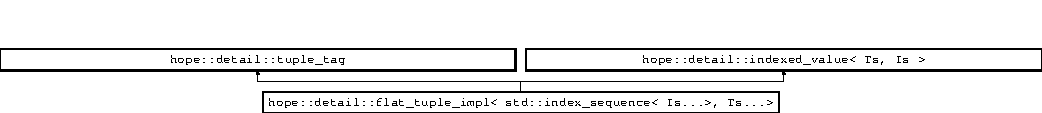
\includegraphics[height=1.48936cm]{classhope_1_1detail_1_1flat__tuple__impl_3_01std_1_1index__sequence_3_01_is_8_8_8_4_00_01_ts_8_8_8_4}
\end{center}
\end{figure}
\subsection*{Public Member Functions}
\begin{CompactItemize}
\item 
{\footnotesize template$<$typename T , typename NativeT  = std::decay\_\-t$<$T$>$$>$ }\\constexpr \hyperlink{classhope_1_1detail_1_1flat__tuple__impl_3_01std_1_1index__sequence_3_01_is_8_8_8_4_00_01_ts_8_8_8_4_6f82e0562ca06b099334fa7c08e0eb64}{decltype} (auto) get() noexcept
\begin{CompactList}\small\item\em Tries to find element of specified type, fails on static assert if element had not been found; method is not sensitive to the qualifiers, followed constructions are equal: get$<$int$>$() get$<$int\&$>$() , get$<$const int$>$(), get$<$const int\&$>$(); accessed value will be automatically deduced by tuple's type (regardless of field policy is being used to create the tuple). \item\end{CompactList}\item 
{\footnotesize template$<$typename T , typename NativeT  = std::decay\_\-t$<$T$>$$>$ }\\constexpr \hyperlink{classhope_1_1detail_1_1flat__tuple__impl_3_01std_1_1index__sequence_3_01_is_8_8_8_4_00_01_ts_8_8_8_4_0db8adfa32e775efc297ffd41fdda6a7}{decltype} (auto) get() const noexcept
\begin{CompactList}\small\item\em Tries to find element of specified type, fails on static assert if element had not been found; method is not sensitive to the qualifiers, followed constructions are equal: get$<$int$>$() get$<$int\&$>$() , get$<$const int$>$(), get$<$const int\&$>$(); accessed value will be automatically deduced by tuple's type (regardless of field policy is being used to create the tuple). \item\end{CompactList}\item 
{\footnotesize template$<$size\_\-t N$>$ }\\constexpr \hyperlink{classhope_1_1detail_1_1flat__tuple__impl_3_01std_1_1index__sequence_3_01_is_8_8_8_4_00_01_ts_8_8_8_4_6f82e0562ca06b099334fa7c08e0eb64}{decltype} (auto) get() noexcept
\begin{CompactList}\small\item\em Tries to find element with given index. \item\end{CompactList}\item 
{\footnotesize template$<$size\_\-t N$>$ }\\constexpr \hyperlink{classhope_1_1detail_1_1flat__tuple__impl_3_01std_1_1index__sequence_3_01_is_8_8_8_4_00_01_ts_8_8_8_4_0db8adfa32e775efc297ffd41fdda6a7}{decltype} (auto) get() const noexcept
\begin{CompactList}\small\item\em Tries to find element with given index. \item\end{CompactList}\item 
{\footnotesize template$<$typename F $>$ }\\constexpr void \hyperlink{classhope_1_1detail_1_1flat__tuple__impl_3_01std_1_1index__sequence_3_01_is_8_8_8_4_00_01_ts_8_8_8_4_666a36927404ca2f5d9faeeb9da9c039}{for\_\-each} (F \&\&f) const 
\begin{CompactList}\small\item\em Applies given functor to each value of tuple, more useful analogue of std::apply. \item\end{CompactList}\item 
{\footnotesize template$<$typename F $>$ }\\constexpr void \hyperlink{classhope_1_1detail_1_1flat__tuple__impl_3_01std_1_1index__sequence_3_01_is_8_8_8_4_00_01_ts_8_8_8_4_217b9226418ab5ac765404e6632a8083}{for\_\-each} (const flat\_\-tuple \&tuple2, F \&\&f) const 
\begin{CompactList}\small\item\em Applies given functor to each value of tuples. \item\end{CompactList}\item 
{\footnotesize template$<$typename F $>$ }\\constexpr void \hyperlink{classhope_1_1detail_1_1flat__tuple__impl_3_01std_1_1index__sequence_3_01_is_8_8_8_4_00_01_ts_8_8_8_4_1ef2389962afceff73d54483975f5628}{for\_\-each} (F \&\&f)
\begin{CompactList}\small\item\em Applies given functor to each value of given tuple, more useful analogue of std::apply. \item\end{CompactList}\item 
{\footnotesize template$<$typename F $>$ }\\constexpr void \hyperlink{classhope_1_1detail_1_1flat__tuple__impl_3_01std_1_1index__sequence_3_01_is_8_8_8_4_00_01_ts_8_8_8_4_90c90aefa83c884fc686a98175d8fcd6}{for\_\-each} (flat\_\-tuple \&tuple2, F \&\&f)
\begin{CompactList}\small\item\em Applies given functor to each value of tuples. \item\end{CompactList}\end{CompactItemize}
\subsection*{Static Public Member Functions}
\begin{CompactItemize}
\item 
static constexpr auto \hyperlink{classhope_1_1detail_1_1flat__tuple__impl_3_01std_1_1index__sequence_3_01_is_8_8_8_4_00_01_ts_8_8_8_4_e8c18d2b32dc3aee7818265152bbfa46}{get\_\-size} () noexcept
\begin{CompactList}\small\item\em just returns the size of the tuple (means number of fields) \item\end{CompactList}\end{CompactItemize}
\subsection*{Protected Member Functions}
\begin{CompactItemize}
\item 
\hypertarget{classhope_1_1detail_1_1flat__tuple__impl_3_01std_1_1index__sequence_3_01_is_8_8_8_4_00_01_ts_8_8_8_4_2c05f9d62b48ab44dbc4493305e58e4e}{
constexpr \textbf{flat\_\-tuple\_\-impl} (const flat\_\-tuple\_\-impl \&)}
\label{classhope_1_1detail_1_1flat__tuple__impl_3_01std_1_1index__sequence_3_01_is_8_8_8_4_00_01_ts_8_8_8_4_2c05f9d62b48ab44dbc4493305e58e4e}

\item 
\hypertarget{classhope_1_1detail_1_1flat__tuple__impl_3_01std_1_1index__sequence_3_01_is_8_8_8_4_00_01_ts_8_8_8_4_095208e9f5ec49ad23353721d69f0868}{
constexpr \textbf{flat\_\-tuple\_\-impl} (flat\_\-tuple\_\-impl \&\&)}
\label{classhope_1_1detail_1_1flat__tuple__impl_3_01std_1_1index__sequence_3_01_is_8_8_8_4_00_01_ts_8_8_8_4_095208e9f5ec49ad23353721d69f0868}

\item 
\hypertarget{classhope_1_1detail_1_1flat__tuple__impl_3_01std_1_1index__sequence_3_01_is_8_8_8_4_00_01_ts_8_8_8_4_583a3a3d9e0227fc5aaf11133d8bd5be}{
{\footnotesize template$<$typename... VTs$>$ }\\constexpr \textbf{flat\_\-tuple\_\-impl} (VTs \&\&...elems) noexcept}
\label{classhope_1_1detail_1_1flat__tuple__impl_3_01std_1_1index__sequence_3_01_is_8_8_8_4_00_01_ts_8_8_8_4_583a3a3d9e0227fc5aaf11133d8bd5be}

\end{CompactItemize}


\subsection{Detailed Description}
\subsubsection*{template$<$std::size\_\-t... Is, typename... Ts$>$ class hope::detail::flat\_\-tuple\_\-impl$<$ std::index\_\-sequence$<$ Is...$>$, Ts...$>$}

General class of the all static reflection module. \begin{Desc}
\item[Template Parameters:]
\begin{description}
\item[{\em Is}]Helper sequence of indexes, max(Is...) + is the count of the tuple's elements \item[{\em Ts}]Types stored in the tuple \end{description}
\end{Desc}


\subsection{Member Function Documentation}
\hypertarget{classhope_1_1detail_1_1flat__tuple__impl_3_01std_1_1index__sequence_3_01_is_8_8_8_4_00_01_ts_8_8_8_4_0db8adfa32e775efc297ffd41fdda6a7}{
\index{hope::detail::flat\_\-tuple\_\-impl$<$ std::index\_\-sequence$<$ Is...$>$, Ts...$>$@{hope::detail::flat\_\-tuple\_\-impl$<$ std::index\_\-sequence$<$ Is...$>$, Ts...$>$}!decltype@{decltype}}
\index{decltype@{decltype}!hope::detail::flat_tuple_impl< std::index_sequence< Is...>, Ts...>@{hope::detail::flat\_\-tuple\_\-impl$<$ std::index\_\-sequence$<$ Is...$>$, Ts...$>$}}
\subsubsection[{decltype}]{\setlength{\rightskip}{0pt plus 5cm}template$<$std::size\_\-t... Is, typename... Ts$>$ template$<$size\_\-t N$>$ constexpr hope::detail::flat\_\-tuple\_\-impl$<$ std::index\_\-sequence$<$ Is...$>$, Ts...$>$::decltype (auto) const\hspace{0.3cm}{\tt  \mbox{[}inline\mbox{]}}}}
\label{classhope_1_1detail_1_1flat__tuple__impl_3_01std_1_1index__sequence_3_01_is_8_8_8_4_00_01_ts_8_8_8_4_0db8adfa32e775efc297ffd41fdda6a7}


Tries to find element with given index. 

\begin{Desc}
\item[Template Parameters:]
\begin{description}
\item[{\em N}]Index of the element to be found \end{description}
\end{Desc}
\begin{Desc}
\item[Returns:]Reference to the containing element, const and ref qualifiers of the containing one do not change, ref will be returned \char`\"{}as is\char`\"{} \end{Desc}
\hypertarget{classhope_1_1detail_1_1flat__tuple__impl_3_01std_1_1index__sequence_3_01_is_8_8_8_4_00_01_ts_8_8_8_4_6f82e0562ca06b099334fa7c08e0eb64}{
\index{hope::detail::flat\_\-tuple\_\-impl$<$ std::index\_\-sequence$<$ Is...$>$, Ts...$>$@{hope::detail::flat\_\-tuple\_\-impl$<$ std::index\_\-sequence$<$ Is...$>$, Ts...$>$}!decltype@{decltype}}
\index{decltype@{decltype}!hope::detail::flat_tuple_impl< std::index_sequence< Is...>, Ts...>@{hope::detail::flat\_\-tuple\_\-impl$<$ std::index\_\-sequence$<$ Is...$>$, Ts...$>$}}
\subsubsection[{decltype}]{\setlength{\rightskip}{0pt plus 5cm}template$<$std::size\_\-t... Is, typename... Ts$>$ template$<$size\_\-t N$>$ constexpr hope::detail::flat\_\-tuple\_\-impl$<$ std::index\_\-sequence$<$ Is...$>$, Ts...$>$::decltype (auto)\hspace{0.3cm}{\tt  \mbox{[}inline\mbox{]}}}}
\label{classhope_1_1detail_1_1flat__tuple__impl_3_01std_1_1index__sequence_3_01_is_8_8_8_4_00_01_ts_8_8_8_4_6f82e0562ca06b099334fa7c08e0eb64}


Tries to find element with given index. 

\begin{Desc}
\item[Template Parameters:]
\begin{description}
\item[{\em N}]Index of the element to be found \end{description}
\end{Desc}
\begin{Desc}
\item[Returns:]Reference to the containing element, const and ref qualifiers of the containing one are not change, ref will be returned \char`\"{}as is\char`\"{} \end{Desc}
\hypertarget{classhope_1_1detail_1_1flat__tuple__impl_3_01std_1_1index__sequence_3_01_is_8_8_8_4_00_01_ts_8_8_8_4_0db8adfa32e775efc297ffd41fdda6a7}{
\index{hope::detail::flat\_\-tuple\_\-impl$<$ std::index\_\-sequence$<$ Is...$>$, Ts...$>$@{hope::detail::flat\_\-tuple\_\-impl$<$ std::index\_\-sequence$<$ Is...$>$, Ts...$>$}!decltype@{decltype}}
\index{decltype@{decltype}!hope::detail::flat_tuple_impl< std::index_sequence< Is...>, Ts...>@{hope::detail::flat\_\-tuple\_\-impl$<$ std::index\_\-sequence$<$ Is...$>$, Ts...$>$}}
\subsubsection[{decltype}]{\setlength{\rightskip}{0pt plus 5cm}template$<$std::size\_\-t... Is, typename... Ts$>$ template$<$typename T , typename NativeT  = std::decay\_\-t$<$T$>$$>$ constexpr hope::detail::flat\_\-tuple\_\-impl$<$ std::index\_\-sequence$<$ Is...$>$, Ts...$>$::decltype (auto) const\hspace{0.3cm}{\tt  \mbox{[}inline\mbox{]}}}}
\label{classhope_1_1detail_1_1flat__tuple__impl_3_01std_1_1index__sequence_3_01_is_8_8_8_4_00_01_ts_8_8_8_4_0db8adfa32e775efc297ffd41fdda6a7}


Tries to find element of specified type, fails on static assert if element had not been found; method is not sensitive to the qualifiers, followed constructions are equal: get$<$int$>$() get$<$int\&$>$() , get$<$const int$>$(), get$<$const int\&$>$(); accessed value will be automatically deduced by tuple's type (regardless of field policy is being used to create the tuple). 

\begin{Desc}
\item[Template Parameters:]
\begin{description}
\item[{\em T}]: Type of element to be returned, const and reference qualifiers does not matter\item[{\em NativeT}]: clear type, used to deduce return type and check whether tuple has element with specified value or not\end{description}
\end{Desc}
\begin{Desc}
\item[Returns:]reference to the containing element \end{Desc}
\hypertarget{classhope_1_1detail_1_1flat__tuple__impl_3_01std_1_1index__sequence_3_01_is_8_8_8_4_00_01_ts_8_8_8_4_6f82e0562ca06b099334fa7c08e0eb64}{
\index{hope::detail::flat\_\-tuple\_\-impl$<$ std::index\_\-sequence$<$ Is...$>$, Ts...$>$@{hope::detail::flat\_\-tuple\_\-impl$<$ std::index\_\-sequence$<$ Is...$>$, Ts...$>$}!decltype@{decltype}}
\index{decltype@{decltype}!hope::detail::flat_tuple_impl< std::index_sequence< Is...>, Ts...>@{hope::detail::flat\_\-tuple\_\-impl$<$ std::index\_\-sequence$<$ Is...$>$, Ts...$>$}}
\subsubsection[{decltype}]{\setlength{\rightskip}{0pt plus 5cm}template$<$std::size\_\-t... Is, typename... Ts$>$ template$<$typename T , typename NativeT  = std::decay\_\-t$<$T$>$$>$ constexpr hope::detail::flat\_\-tuple\_\-impl$<$ std::index\_\-sequence$<$ Is...$>$, Ts...$>$::decltype (auto)\hspace{0.3cm}{\tt  \mbox{[}inline\mbox{]}}}}
\label{classhope_1_1detail_1_1flat__tuple__impl_3_01std_1_1index__sequence_3_01_is_8_8_8_4_00_01_ts_8_8_8_4_6f82e0562ca06b099334fa7c08e0eb64}


Tries to find element of specified type, fails on static assert if element had not been found; method is not sensitive to the qualifiers, followed constructions are equal: get$<$int$>$() get$<$int\&$>$() , get$<$const int$>$(), get$<$const int\&$>$(); accessed value will be automatically deduced by tuple's type (regardless of field policy is being used to create the tuple). 

\begin{Desc}
\item[Template Parameters:]
\begin{description}
\item[{\em T}]: Type of element to be returned, const and reference qualifiers does not matter\item[{\em NativeT}]: clear type, used to deduce return type and check whether tuple has element with specified value or not\end{description}
\end{Desc}
\begin{Desc}
\item[Returns:]reference to the containing element \end{Desc}
\hypertarget{classhope_1_1detail_1_1flat__tuple__impl_3_01std_1_1index__sequence_3_01_is_8_8_8_4_00_01_ts_8_8_8_4_90c90aefa83c884fc686a98175d8fcd6}{
\index{hope::detail::flat\_\-tuple\_\-impl$<$ std::index\_\-sequence$<$ Is...$>$, Ts...$>$@{hope::detail::flat\_\-tuple\_\-impl$<$ std::index\_\-sequence$<$ Is...$>$, Ts...$>$}!for\_\-each@{for\_\-each}}
\index{for\_\-each@{for\_\-each}!hope::detail::flat_tuple_impl< std::index_sequence< Is...>, Ts...>@{hope::detail::flat\_\-tuple\_\-impl$<$ std::index\_\-sequence$<$ Is...$>$, Ts...$>$}}
\subsubsection[{for\_\-each}]{\setlength{\rightskip}{0pt plus 5cm}template$<$std::size\_\-t... Is, typename... Ts$>$ template$<$typename F $>$ constexpr void hope::detail::flat\_\-tuple\_\-impl$<$ std::index\_\-sequence$<$ Is...$>$, Ts...$>$::for\_\-each (flat\_\-tuple \& {\em tuple2}, \/  F \&\& {\em f})\hspace{0.3cm}{\tt  \mbox{[}inline\mbox{]}}}}
\label{classhope_1_1detail_1_1flat__tuple__impl_3_01std_1_1index__sequence_3_01_is_8_8_8_4_00_01_ts_8_8_8_4_90c90aefa83c884fc686a98175d8fcd6}


Applies given functor to each value of tuples. 

\begin{Desc}
\item[Template Parameters:]
\begin{description}
\item[{\em F}]type of functional object \end{description}
\end{Desc}
\begin{Desc}
\item[Parameters:]
\begin{description}
\item[{\em tuple2}]second tuple the function to be applied to \item[{\em f}]functional object to be sequentially applied to each field of tuple \end{description}
\end{Desc}
\hypertarget{classhope_1_1detail_1_1flat__tuple__impl_3_01std_1_1index__sequence_3_01_is_8_8_8_4_00_01_ts_8_8_8_4_1ef2389962afceff73d54483975f5628}{
\index{hope::detail::flat\_\-tuple\_\-impl$<$ std::index\_\-sequence$<$ Is...$>$, Ts...$>$@{hope::detail::flat\_\-tuple\_\-impl$<$ std::index\_\-sequence$<$ Is...$>$, Ts...$>$}!for\_\-each@{for\_\-each}}
\index{for\_\-each@{for\_\-each}!hope::detail::flat_tuple_impl< std::index_sequence< Is...>, Ts...>@{hope::detail::flat\_\-tuple\_\-impl$<$ std::index\_\-sequence$<$ Is...$>$, Ts...$>$}}
\subsubsection[{for\_\-each}]{\setlength{\rightskip}{0pt plus 5cm}template$<$std::size\_\-t... Is, typename... Ts$>$ template$<$typename F $>$ constexpr void hope::detail::flat\_\-tuple\_\-impl$<$ std::index\_\-sequence$<$ Is...$>$, Ts...$>$::for\_\-each (F \&\& {\em f})\hspace{0.3cm}{\tt  \mbox{[}inline\mbox{]}}}}
\label{classhope_1_1detail_1_1flat__tuple__impl_3_01std_1_1index__sequence_3_01_is_8_8_8_4_00_01_ts_8_8_8_4_1ef2389962afceff73d54483975f5628}


Applies given functor to each value of given tuple, more useful analogue of std::apply. 

\begin{Desc}
\item[Template Parameters:]
\begin{description}
\item[{\em F}]type of functional object \end{description}
\end{Desc}
\begin{Desc}
\item[Parameters:]
\begin{description}
\item[{\em f}]functional object to be sequentially applied to each field of tuple \end{description}
\end{Desc}
\hypertarget{classhope_1_1detail_1_1flat__tuple__impl_3_01std_1_1index__sequence_3_01_is_8_8_8_4_00_01_ts_8_8_8_4_217b9226418ab5ac765404e6632a8083}{
\index{hope::detail::flat\_\-tuple\_\-impl$<$ std::index\_\-sequence$<$ Is...$>$, Ts...$>$@{hope::detail::flat\_\-tuple\_\-impl$<$ std::index\_\-sequence$<$ Is...$>$, Ts...$>$}!for\_\-each@{for\_\-each}}
\index{for\_\-each@{for\_\-each}!hope::detail::flat_tuple_impl< std::index_sequence< Is...>, Ts...>@{hope::detail::flat\_\-tuple\_\-impl$<$ std::index\_\-sequence$<$ Is...$>$, Ts...$>$}}
\subsubsection[{for\_\-each}]{\setlength{\rightskip}{0pt plus 5cm}template$<$std::size\_\-t... Is, typename... Ts$>$ template$<$typename F $>$ constexpr void hope::detail::flat\_\-tuple\_\-impl$<$ std::index\_\-sequence$<$ Is...$>$, Ts...$>$::for\_\-each (const flat\_\-tuple \& {\em tuple2}, \/  F \&\& {\em f}) const\hspace{0.3cm}{\tt  \mbox{[}inline\mbox{]}}}}
\label{classhope_1_1detail_1_1flat__tuple__impl_3_01std_1_1index__sequence_3_01_is_8_8_8_4_00_01_ts_8_8_8_4_217b9226418ab5ac765404e6632a8083}


Applies given functor to each value of tuples. 

\begin{Desc}
\item[Template Parameters:]
\begin{description}
\item[{\em F}]type of functional object \end{description}
\end{Desc}
\begin{Desc}
\item[Parameters:]
\begin{description}
\item[{\em tuple2}]second tuple the function to be applied to \item[{\em f}]functional object to be sequentially applied to each field of tuple \end{description}
\end{Desc}
\hypertarget{classhope_1_1detail_1_1flat__tuple__impl_3_01std_1_1index__sequence_3_01_is_8_8_8_4_00_01_ts_8_8_8_4_666a36927404ca2f5d9faeeb9da9c039}{
\index{hope::detail::flat\_\-tuple\_\-impl$<$ std::index\_\-sequence$<$ Is...$>$, Ts...$>$@{hope::detail::flat\_\-tuple\_\-impl$<$ std::index\_\-sequence$<$ Is...$>$, Ts...$>$}!for\_\-each@{for\_\-each}}
\index{for\_\-each@{for\_\-each}!hope::detail::flat_tuple_impl< std::index_sequence< Is...>, Ts...>@{hope::detail::flat\_\-tuple\_\-impl$<$ std::index\_\-sequence$<$ Is...$>$, Ts...$>$}}
\subsubsection[{for\_\-each}]{\setlength{\rightskip}{0pt plus 5cm}template$<$std::size\_\-t... Is, typename... Ts$>$ template$<$typename F $>$ constexpr void hope::detail::flat\_\-tuple\_\-impl$<$ std::index\_\-sequence$<$ Is...$>$, Ts...$>$::for\_\-each (F \&\& {\em f}) const\hspace{0.3cm}{\tt  \mbox{[}inline\mbox{]}}}}
\label{classhope_1_1detail_1_1flat__tuple__impl_3_01std_1_1index__sequence_3_01_is_8_8_8_4_00_01_ts_8_8_8_4_666a36927404ca2f5d9faeeb9da9c039}


Applies given functor to each value of tuple, more useful analogue of std::apply. 

\begin{Desc}
\item[Template Parameters:]
\begin{description}
\item[{\em F}]type of functional object \end{description}
\end{Desc}
\begin{Desc}
\item[Parameters:]
\begin{description}
\item[{\em f}]functional object to be sequentially applied to each field of tuple \end{description}
\end{Desc}
\hypertarget{classhope_1_1detail_1_1flat__tuple__impl_3_01std_1_1index__sequence_3_01_is_8_8_8_4_00_01_ts_8_8_8_4_e8c18d2b32dc3aee7818265152bbfa46}{
\index{hope::detail::flat\_\-tuple\_\-impl$<$ std::index\_\-sequence$<$ Is...$>$, Ts...$>$@{hope::detail::flat\_\-tuple\_\-impl$<$ std::index\_\-sequence$<$ Is...$>$, Ts...$>$}!get\_\-size@{get\_\-size}}
\index{get\_\-size@{get\_\-size}!hope::detail::flat_tuple_impl< std::index_sequence< Is...>, Ts...>@{hope::detail::flat\_\-tuple\_\-impl$<$ std::index\_\-sequence$<$ Is...$>$, Ts...$>$}}
\subsubsection[{get\_\-size}]{\setlength{\rightskip}{0pt plus 5cm}template$<$std::size\_\-t... Is, typename... Ts$>$ static constexpr auto hope::detail::flat\_\-tuple\_\-impl$<$ std::index\_\-sequence$<$ Is...$>$, Ts...$>$::get\_\-size ()\hspace{0.3cm}{\tt  \mbox{[}inline, static\mbox{]}}}}
\label{classhope_1_1detail_1_1flat__tuple__impl_3_01std_1_1index__sequence_3_01_is_8_8_8_4_00_01_ts_8_8_8_4_e8c18d2b32dc3aee7818265152bbfa46}


just returns the size of the tuple (means number of fields) 

\begin{Desc}
\item[Returns:]number of fields \end{Desc}


The documentation for this class was generated from the following file:\begin{CompactItemize}
\item 
lib/hope/tuple/\hyperlink{flat__tuple_8h}{flat\_\-tuple.h}\end{CompactItemize}

\hypertarget{structhope_1_1detail_1_1indexed__value}{}\doxysection{hope\+::detail\+::indexed\+\_\+value\texorpdfstring{$<$}{<} T, I \texorpdfstring{$>$}{>} Struct Template Reference}
\label{structhope_1_1detail_1_1indexed__value}\index{hope::detail::indexed\_value$<$ T, I $>$@{hope::detail::indexed\_value$<$ T, I $>$}}
\doxysubsection*{Public Member Functions}
\begin{DoxyCompactItemize}
\item 
\mbox{\Hypertarget{structhope_1_1detail_1_1indexed__value_ac753cdc76a4e75e83d717855b376d05b}\label{structhope_1_1detail_1_1indexed__value_ac753cdc76a4e75e83d717855b376d05b}} 
constexpr {\bfseries indexed\+\_\+value} (\mbox{\hyperlink{structhope_1_1detail_1_1indexed__value}{indexed\+\_\+value}} \&\&)=default
\item 
\mbox{\Hypertarget{structhope_1_1detail_1_1indexed__value_a9bb86190fc0226560513a5c3a46b1fb9}\label{structhope_1_1detail_1_1indexed__value_a9bb86190fc0226560513a5c3a46b1fb9}} 
constexpr {\bfseries indexed\+\_\+value} (const \mbox{\hyperlink{structhope_1_1detail_1_1indexed__value}{indexed\+\_\+value}} \&)=default
\item 
\mbox{\Hypertarget{structhope_1_1detail_1_1indexed__value_a90e3b2c62118274b207ff807558116ef}\label{structhope_1_1detail_1_1indexed__value_a90e3b2c62118274b207ff807558116ef}} 
{\footnotesize template$<$typename Vt , typename  = std\+::is\+\_\+constructible$<$\+T, Vt$>$$>$ }\\constexpr {\bfseries indexed\+\_\+value} (Vt \&\&value\+Ref)
\end{DoxyCompactItemize}
\doxysubsection*{Public Attributes}
\begin{DoxyCompactItemize}
\item 
\mbox{\Hypertarget{structhope_1_1detail_1_1indexed__value_ab07effb8e8df844a470f645393f55fc5}\label{structhope_1_1detail_1_1indexed__value_ab07effb8e8df844a470f645393f55fc5}} 
T {\bfseries value}
\end{DoxyCompactItemize}


The documentation for this struct was generated from the following file\+:\begin{DoxyCompactItemize}
\item 
lib/hope/tuple/flat\+\_\+tuple.\+h\end{DoxyCompactItemize}

\hypertarget{classhope_1_1memory_1_1small__object}{
\section{hope::memory::small\_\-object Class Reference}
\label{classhope_1_1memory_1_1small__object}\index{hope::memory::small\_\-object@{hope::memory::small\_\-object}}
}
thin useful wrapper of small\_\-object\_\-allocator just inherit your class from this, and u get height quality boost of performance :) take safe and fasten seat belts, the rocket starts now!  


{\tt \#include $<$small\_\-object.h$>$}

\subsection*{Public Member Functions}
\begin{CompactItemize}
\item 
\hypertarget{classhope_1_1memory_1_1small__object_d91fb7945fdefd0052d9f51128aaf5ed}{
void $\ast$ \textbf{operator new} (std::size\_\-t size)}
\label{classhope_1_1memory_1_1small__object_d91fb7945fdefd0052d9f51128aaf5ed}

\item 
\hypertarget{classhope_1_1memory_1_1small__object_6d6af0257cd010419871f45b2d8aedf9}{
void \textbf{operator delete} (void $\ast$ptr, std::size\_\-t size)}
\label{classhope_1_1memory_1_1small__object_6d6af0257cd010419871f45b2d8aedf9}

\end{CompactItemize}


\subsection{Detailed Description}
thin useful wrapper of small\_\-object\_\-allocator just inherit your class from this, and u get height quality boost of performance :) take safe and fasten seat belts, the rocket starts now! 

The documentation for this class was generated from the following files:\begin{CompactItemize}
\item 
lib/hope/memory/small\_\-object/small\_\-object.h\item 
lib/hope/memory/small\_\-object/small\_\-object.cpp\end{CompactItemize}

\hypertarget{structhope_1_1detail_1_1tuple__tag}{}\doxysection{hope\+::detail\+::tuple\+\_\+tag Struct Reference}
\label{structhope_1_1detail_1_1tuple__tag}\index{hope::detail::tuple\_tag@{hope::detail::tuple\_tag}}


Tag is used to identify whether object of provided type is tuple or not.  




{\ttfamily \#include $<$flat\+\_\+tuple.\+h$>$}

Inheritance diagram for hope\+::detail\+::tuple\+\_\+tag\+:\begin{figure}[H]
\begin{center}
\leavevmode
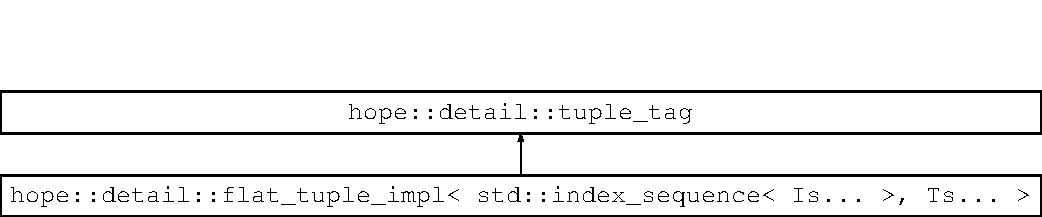
\includegraphics[height=2.000000cm]{structhope_1_1detail_1_1tuple__tag}
\end{center}
\end{figure}


\doxysubsection{Detailed Description}
Tag is used to identify whether object of provided type is tuple or not. 

The documentation for this struct was generated from the following file\+:\begin{DoxyCompactItemize}
\item 
lib/hope/tuple/flat\+\_\+tuple.\+h\end{DoxyCompactItemize}

\chapter{File Documentation}
\hypertarget{compute__field__count__recursive_8h}{
\section{lib/hope/tuple/compute\_\-field\_\-count\_\-recursive.h File Reference}
\label{compute__field__count__recursive_8h}\index{lib/hope/tuple/compute\_\-field\_\-count\_\-recursive.h@{lib/hope/tuple/compute\_\-field\_\-count\_\-recursive.h}}
}
the file contains several functions for recursively calculating the number of fields within the structure. Only user-defined types are computed recursively, the classes of the standard library are considered a single whole  


{\tt \#include \char`\"{}hope/tuple/tuple\_\-from\_\-struct.h\char`\"{}}\par
{\tt \#include \char`\"{}hope/tuple/tuple\_\-from\_\-struct\_\-unsafe.h\char`\"{}}\par
{\tt \#include \char`\"{}hope/tuple/tuple\_\-policy.h\char`\"{}}\par
{\tt \#include \char`\"{}hope/components/user\_\-defined\_\-types.h\char`\"{}}\par
{\tt \#include \char`\"{}hope/components/detector.h\char`\"{}}\par
\subsection*{Functions}
\begin{CompactItemize}
\item 
{\footnotesize template$<$typename TStructure $>$ }\\constexpr std::size\_\-t \hyperlink{namespacehope_d888d2898671bf971a6fc36ad009f5fd}{hope::compute\_\-field\_\-count\_\-recursive\_\-constexpr} ()
\item 
{\footnotesize template$<$typename TStructure $>$ }\\std::size\_\-t \hyperlink{namespacehope_d80c3f26e3739b22af3cfa9a99400d9f}{hope::compute\_\-field\_\-count\_\-recursive} ()
\end{CompactItemize}


\subsection{Detailed Description}
the file contains several functions for recursively calculating the number of fields within the structure. Only user-defined types are computed recursively, the classes of the standard library are considered a single whole 


\hypertarget{detect__fields__count_8h}{
\section{lib/hope/tuple/detect\_\-fields\_\-count.h File Reference}
\label{detect__fields__count_8h}\index{lib/hope/tuple/detect\_\-fields\_\-count.h@{lib/hope/tuple/detect\_\-fields\_\-count.h}}
}
This file consists of helper functions which is used to compute fields count (in general) And the only one function which computes count of the structure's fields (non - recursive).  


{\tt \#include $<$utility$>$}\par
\subsection*{Classes}
\begin{CompactItemize}
\item 
struct \hyperlink{structhope_1_1detail_1_1any__convertible}{hope::detail::any\_\-convertible$<$ TStruct, I $>$}
\end{CompactItemize}
\subsection*{Functions}
\begin{CompactItemize}
\item 
{\footnotesize template$<$typename TStruct , std::size\_\-t... Is$>$ }\\constexpr auto \hyperlink{namespacehope_1_1detail_cc4c5423da0368a154408a209834b6a7}{hope::detail::is\_\-constructable\_\-n} (std::index\_\-sequence$<$ Is...$>$) $\rightarrow$ decltype(TStruct
\item 
\hypertarget{namespacehope_1_1detail_0c48744cad1f53ece8076378360d143b}{
\textbf{hope::detail::bool} ())}
\label{namespacehope_1_1detail_0c48744cad1f53ece8076378360d143b}

\item 
\hypertarget{namespacehope_1_1detail_ce142bbc3d81f75264bc58dd6029b34b}{
{\footnotesize template$<$typename TStruct , std::size\_\-t... Is$>$ }\\constexpr auto \textbf{hope::detail::is\_\-constructable\_\-n} (...)}
\label{namespacehope_1_1detail_ce142bbc3d81f75264bc58dd6029b34b}

\item 
{\footnotesize template$<$typename TStructure , std::size\_\-t... Is$>$ }\\constexpr std::size\_\-t \hyperlink{namespacehope_1_1detail_a2afda571bf78d30c1e1e9d1a52d1e12}{hope::detail::detect\_\-fields\_\-count\_\-impl} (std::index\_\-sequence$<$ Is...$>$ sequence)
\item 
{\footnotesize template$<$typename TStructure $>$ }\\constexpr std::size\_\-t \hyperlink{namespacehope_0357aa16dc8ddf9ddd4d4aacd93fbcf3}{hope::detect\_\-fields\_\-count} ()
\end{CompactItemize}


\subsection{Detailed Description}
This file consists of helper functions which is used to compute fields count (in general) And the only one function which computes count of the structure's fields (non - recursive). 


\hypertarget{flat__sorted__tuple_8h}{
\section{lib/hope/tuple/flat\_\-sorted\_\-tuple.h File Reference}
\label{flat__sorted__tuple_8h}\index{lib/hope/tuple/flat\_\-sorted\_\-tuple.h@{lib/hope/tuple/flat\_\-sorted\_\-tuple.h}}
}
This file contains function which might be used to create tuple of specified types. Before tuple creation all the corresponding types sorts and reorders by predicate.  


{\tt \#include \char`\"{}hope/typelist/type\_\-list.h\char`\"{}}\par
{\tt \#include \char`\"{}hope/typelist/typelistsort.h\char`\"{}}\par
{\tt \#include \char`\"{}hope/tuple/flat\_\-tuple.h\char`\"{}}\par
\subsection*{Functions}
\begin{CompactItemize}
\item 
\hypertarget{namespacehope_1_1detail_92f958a639802111c3ca5c19efd66407}{
{\footnotesize template$<$typename... Ts, typename... Vs$>$ }\\constexpr auto \textbf{hope::detail::make\_\-flat\_\-tuple\_\-from\_\-type\_\-list} (type\_\-list$<$ Ts...$>$, Vs \&\&...args)}
\label{namespacehope_1_1detail_92f958a639802111c3ca5c19efd66407}

\item 
{\footnotesize template$<$typename... Ts$>$ }\\constexpr auto \hyperlink{namespacehope_4d5d6cdd0a3c59e7e6d3f9036bf3d135}{hope::make\_\-sorted\_\-tuple} (Ts \&\&...args)
\end{CompactItemize}


\subsection{Detailed Description}
This file contains function which might be used to create tuple of specified types. Before tuple creation all the corresponding types sorts and reorders by predicate. 


\hypertarget{flat__tuple_8h}{
\section{lib/hope/tuple/flat\_\-tuple.h File Reference}
\label{flat__tuple_8h}\index{lib/hope/tuple/flat\_\-tuple.h@{lib/hope/tuple/flat\_\-tuple.h}}
}
Implementation of non - recursive tuple, tuple size and alignment is same as structure with fields of specified types; Also this class contains a lot of useful methods.  


{\tt \#include \char`\"{}hope/typelist/type\_\-list.h\char`\"{}}\par
{\tt \#include \char`\"{}hope/foundation.h\char`\"{}}\par
\subsection*{Classes}
\begin{CompactItemize}
\item 
struct \hyperlink{structhope_1_1detail_1_1tuple__tag}{hope::detail::tuple\_\-tag}
\begin{CompactList}\small\item\em Tag is used to identify whether object of provided type is tuple or not. \item\end{CompactList}\item 
struct \hyperlink{structhope_1_1detail_1_1indexed__value}{hope::detail::indexed\_\-value$<$ T, I $>$}
\item 
class \hyperlink{classhope_1_1detail_1_1flat__tuple__impl_3_01std_1_1index__sequence_3_01_is_8_8_8_4_00_01_ts_8_8_8_4}{hope::detail::flat\_\-tuple\_\-impl$<$ std::index\_\-sequence$<$ Is...$>$, Ts...$>$}
\item 
class \hyperlink{classhope_1_1final}{hope::final$<$ T $>$}
\begin{CompactList}\small\item\em Implementation of the struct like non recursive tuple which might be used to directly cast to struct with same fields because alignment of the structs's fields and tuple's fields are match. \item\end{CompactList}\end{CompactItemize}
\subsection*{Functions}
\begin{CompactItemize}
\item 
\hypertarget{namespacehope_ee3c0903c9de52ddea6f49cb8e1690ee}{
{\footnotesize template$<$typename... Ts$>$ }\\\textbf{hope::flat\_\-tuple} (Ts...) $\rightarrow$ flat\_\-tuple$<$ Ts...$>$}
\label{namespacehope_ee3c0903c9de52ddea6f49cb8e1690ee}

\item 
{\footnotesize template$<$typename... Ts$>$ }\\constexpr auto \hyperlink{namespacehope_3e8db7eca5158658951d01fe4773452b}{hope::make\_\-flat\_\-tuple} (Ts \&\&...args)
\begin{CompactList}\small\item\em Helper function, which should be used to create flat tuple with given arguments all given values will be forwarded to the tuple instance. \item\end{CompactList}\item 
{\footnotesize template$<$typename... Ts$>$ }\\constexpr auto \hyperlink{namespacehope_5d72b1e4164aa5ec2b624f45e6770f35}{hope::make\_\-flat\_\-tuple\_\-bitfield\_\-friendly} (Ts...args)
\begin{CompactList}\small\item\em Helper function, should be used to create tuple of elements with specified bit size. \item\end{CompactList}\item 
{\footnotesize template$<$typename... Ts$>$ }\\constexpr auto \hyperlink{namespacehope_5c5a9595f11522d03c4e2d41ba79f66b}{hope::make\_\-flat\_\-ref\_\-tuple} (Ts \&\&...args)
\begin{CompactList}\small\item\em Helper function, creates tuple with references to the given arguments; const quality of arguments do not changes. \item\end{CompactList}\end{CompactItemize}


\subsection{Detailed Description}
Implementation of non - recursive tuple, tuple size and alignment is same as structure with fields of specified types; Also this class contains a lot of useful methods. 


\hypertarget{print__tuple_8h}{
\section{lib/hope/tuple/print\_\-tuple.h File Reference}
\label{print__tuple_8h}\index{lib/hope/tuple/print\_\-tuple.h@{lib/hope/tuple/print\_\-tuple.h}}
}
Implementation of helper print functions. This functions might be used to print any instance of the aggregate type to the output stream; File contains a quit heavy include : iostream and should never be included at the header. Be careful with usages of these operators.  


{\tt \#include \char`\"{}hope/tuple/flat\_\-tuple.h\char`\"{}}\par
{\tt \#include \char`\"{}hope/tuple/tuple\_\-from\_\-struct.h\char`\"{}}\par
{\tt \#include $<$iostream$>$}\par
\subsection*{Functions}
\begin{CompactItemize}
\item 
{\footnotesize template$<$typename... Ts, std::size\_\-t... VIs$>$ }\\void \hyperlink{namespacehope_1_1detail_7c18953cbf0db2a28a7acacbec941be9}{hope::detail::print\_\-impl} (std::ostream \&stream, const flat\_\-tuple$<$ Ts...$>$ \&tuple, std::index\_\-sequence$<$ VIs...$>$)
\item 
{\footnotesize template$<$typename... Ts$>$ }\\constexpr std::ostream \& \hyperlink{namespacehope_f1dd9390573623b048f5c64caef7327f}{hope::operator$<$$<$} (std::ostream \&stream, const flat\_\-tuple$<$ Ts...$>$ \&tuple)
\item 
{\footnotesize template$<$typename T $>$ }\\constexpr std::ostream \& \hyperlink{group__reflection_gbd3ce49df2aedd37c653a40d28c15b2f}{operator$<$$<$} (std::ostream \&stream, const T \&object)
\end{CompactItemize}


\subsection{Detailed Description}
Implementation of helper print functions. This functions might be used to print any instance of the aggregate type to the output stream; File contains a quit heavy include : iostream and should never be included at the header. Be careful with usages of these operators. 


\printindex
\end{document}
